%\device{postscript}
%\make{manual}
%\disable{figurecontents}
%\libraryfile{Garnet}
%\string{TitleString = `Garnet Tutorial'}
%\use{Bibliography = `garnet.bib'}

\begin{titlepage}
%\begin{titlebox}
\vspace{0.6in}

\begin{center} 

\Large{\textbf{Garnet Tutorial}} \\

\large{{\bf Andrew Mickish}}  \\
\textbf{Revised and translated to LaTeX by Robert P. Goldman}\\

%\vspace{0.3in} 
\today{} \\
{\bf Abstract}
\end{center}
  % \begin{text}
  This tutorial has been designed to introduce the reader to the basic
  concepts of Garnet.  The reader should have already taken the Garnet
  Tour before starting the tutorial.
  \vspace{\fill}
  \begin{center}
Copyright \j{w} 1990 - Carnegie Mellon University\end{center}

This research was sponsored by the Defense Advanced Research Projects
Agency (DOD), ARPA Order No. 4976, Amendment 20, under contract
F33615-87-C-1499,
monitored by the Avionics Laboratory, Air Force Wright Aeronautical
Laboratories, Aeronautical Systems Division (AFSC), Wright-Patterson AFB,
Ohio 45433-6543.

The views and conclusions contained in this document are
those of the authors and should not be interpreted as representing the
official policies, either expressed or implied, of the Defense Advanced
Research Projects Agency or the US Government.


  Many thanks to Ross Moore for helpful advice in translating this
  document into HTML using Latex2HTML.

\end{titlepage}

\tableofcontents{}


% \string{overview = `1'} % \comment{26 pages}
\string{overview-first-page = `3'}
\string{apps = `27'} % \comment{12 pages}
\string{apps-first-page = `29'}
\string{tour = `41'} % \comment{20 pages}
\string{tour-first-page = `43'}
\string{tutorial = `61'} % \comment{42 pages}
\string{tutorial-first-page = `63'}
\string{kr = `101'} % \comment{52 pages}
\string{kr-first-page = `103'}
\string{opal = `151'} % \comment{70 pages}
\string{opal-first-page = `153'}
\string{inter = `219'} % \comment{78 pages}
\string{inter-first-page = `221'}
\string{aggregadgets = `295'} % \comment{54 pages}
\string{aggregadgets-first-page = `297'}
\string{gadgets = `347'} % \comment{116 pages}
\string{gadgets-first-page = `349'}
\string{debug = `461'} % \comment{20 pages}
\string{debug-first-page = `463'}
\string{demos = `481'} % \comment{10 pages}
\string{demos-first-page = `483'}
\string{sampleprog = `491'} % \comment{14 pages}
\string{sampleprog-first-page = `493'}
\string{gilt = `505'} % \comment{20 pages}
\string{gilt-first-page = `507'}
\string{c32 = `525'} % \comment{12 pages}
\string{c32-first-page = `527'}
\string{lapidary = `537'} % \comment{36 pages}
\string{lapidary-first-page = `539'}
\string{hints = `573'} % \comment{8 pages}
\string{hints-first-page = `575'}
\string{GlobalIndex = `580'}

% \set{page = tutorial-first-page}

\chapter{Setting Up}

\section{Take the Tour}

Before beginning this tutorial, you should have already completed the
Garnet Tour, available in a separate document.  The Tour was a series
of exercises intended to acquaint you with a few of the features of
Garnet, while giving you a feel for the interactive programming aspects
of Garnet.  This Tutorial investigates all of those features in
greater depth, while explaining the fundamental principles behind
objects, inheritance, constraints, interactors, and the actual writing
of code.

In the Garnet Tour, you were given some background information about
how to load Garnet, how to access the different Garnet packages,
garbage collection, the main-event-loop for interactors, etc.  It may
be helpful to review this information from the first few sections of
the Tour before starting the Tutorial.


\section{Load Garnet}

Using the instructions from the Tour, load Garnet into your lisp
process.  Also, type in the following line so that references to
the KR package can be eliminated (we will explicitly reference the
other Garnet packages):

\begin{programexample}
(use-package :KR)
\end{programexample}


\chapter{The Prototype-Instance System}

The basic idea behind programming in Garnet is creating objects
and displaying them in windows on the screen.
An object is any of the fundamental data types in Garnet.  Lines,
circles, aggregates and windows are all objects.  These are all
{\it prototype} objects -- you make copies of these objects and
customize the copies to have your desired size and position, as well
as other graphic qualities such as filling styles and line styles.
When you make a customized copy of an object, we say you create an
{\it instance} of the object.  Thus, Garnet is a prototype-instance system.


\section{Inheritance}
\label{inheritance}

When instances are created, an inheritance link is established between
the prototype and the instance.  {\it Inheritance} is the property that
allows instances to get values from their prototypes without specifying
those values in the instances themselves.  For example, if we set the
filling style of a rectangle to be gray, and then we create an
instance of that rectangle, then the instance will also have a gray
filling style.  Naturally, this leads to an inheritance hierarchy
among the objects in the Garnet system.
In fact, there is one root object in Garnet -- the \pr{view-object} -- that
all other objects are instances of (except for interactors, which have
their own root).  Figure \ref{opalInheritance}
shows some of the objects in Garnet and how they fit into the
inheritance hierarchy.  (The average user will never be concerned with
the actual \pr{view-object} or \pr{graphical-object} prototypes.)

% \begin{group}
% \bar{}
\begin{figure}
  \begin{center}
\begin{makeimage}
\end{makeimage}
\begin{latexonly}
    \epsfig{file=opal-inheritance.ps,width=.9\textwidth}
\end{latexonly}
    \htmladdimg{../gifs/opal-inheritance.gif}
  \end{center}
\caption{The inheritance hierarchy among some of the Garnet prototype objects.
All of the standard shapes in garnet are instances of the
\pr{graphical-object} prototype.  As an example of inheritance, the
\pr{circle} and \pr{oval} objects are both special types of arcs, and
they inherit most of their properties from the \pr{arc} prototype
object.  The Gadgets (the Garnet widgets) are not pictured in this
hierarchy, but most of them are instances of the \pr{aggregadget} object.}
\tag{opalInheritance}
%\bar{}
\end{figure}
%\end{group}
%\vspace{1 line}

%\begin{group}
To see an example of inheritance, let's create an instance of a window
and look at some of its inherited values.  After you have loaded Garnet,
type in the following code.

\begin{programexample}
(create-instance 'MY-WIN inter:interactor-window
   (:left 800) (:top 100))
(opal:update MY-WIN)  {\it ; To make the window appear}
\end{programexample}
%\end{group}
%\vspace{1 line}

The window should appear in the upper-right corner of your screen.
In the definition of the MY-WIN schema, we gave a value of 800 to the
\pr{:left} slot and a value of 100 to the \pr{:top} slot.  Let's check
these slots in MY-WIN to see if they are correct.  Type in the
following lines.

\begin{programexample}
(gv MY-WIN :left)    {\it ; Should be 800}
(gv MY-WIN :top)     {\it ; Should be 100}
\end{programexample}

The function \pr{gv} gets the values of slots from an object.
If you got the right values for the \pr{:left} and \pr{:top} slots of
MY-WIN, then you see that the values you supplied during the
\pr{create-instance} call are still being used by MY-WIN.  These are values
that are held in the instance itself.  On the other hand, try typing
in the following lines.

\begin{programexample}
(gv MY-WIN :width)
(gv MY-WIN :height)
\end{programexample}

We did not supply values to the \pr{:width} and \pr{:height} slots of
MY-WIN when it was created.  Therefore, these values are {\it inherited}
from the prototype.  That is, they were defined in the
\pr{interactor-window} object when it was created, and now MY-WIN
inherits those values as its own.  We could, however, override these
inherited values.  Let's change the width and height of MY-WIN using
\pr{s-value}, the function that sets the values of slots.

\begin{programexample}
(s-value MY-WIN :width 100)
(s-value MY-WIN :height 400)
(opal:update MY-WIN)  {\it ; To cause the changes to appear}
\end{programexample}

The dimensions of the window should change, reflecting the new values
we have supplied to its \pr{:width} and \pr{:height} slots.  If we
were to now use \pr{gv} to look at the width and height of
MY-WIN, we would get back the new values, since the old ones are no
longer inherited.

The inheritance hierarchy which was partially pictured in Figure
\ref{opalInheritance} is traced from the leaves toward the root
(from right to left) during a search for a value.
Whenever we use \pr{gv} to get the value of a slot, the object
first checks to see if it has a local value for that slot.  If there
is no value for the slot in the object, then the object looks to its
prototype to see if it has a value for the slot.  This search
continues until either a value for the slot is found or the root
object is reached.  When no inherited or local value for the slot is
found, the value NIL is returned (which, by the way, looks just the
same as a user-defined local value of NIL for a slot).

Since we are now finished with the example of MY-WIN, let's destroy it
so it does not interfere with future examples in this tutorial.  Type
in the following line.

\begin{programexample}
(opal:destroy MY-WIN)
\end{programexample}


\section{Prototypes}
\label{prototypes}

When programming in Garnet, inheritance among objects can eliminate a
lot of duplicated code.  If we want to create several objects that
look similar, we could create each of them from scratch and copy all
the values that we need into each object.  However, inheritance allows
us to define these objects more efficiently, by creating several
similar objects as instances of a single prototype.

\begin{figure}
%\bar{}
  \begin{center}
\begin{makeimage}
\end{makeimage}
\begin{latexonly}
    \epsfig{file=proto-rects.ps}
\end{latexonly}
    \htmladdimg{../gifs/proto-rects.gif}
  \end{center}
\caption{Three instances created from one prototype rectangle.}
\tag{protoRects}
\end{figure}

To start, look at the picture in Figure \ref{protoRects}.  We are
going to define three rectangles with three different filling styles
and put them in a window.  First, let's create a window with a
top-level aggregate.  (For now, just think of an aggregate as an
object which contains several other objects.)  As we add our objects
to this aggregate, they will be displayed in the window.

\begin{programexample}
(create-instance 'WIN inter:interactor-window
   (:left 750)(:top 80)(:width 200)(:height 400))
(create-instance 'TOP-AGG opal:aggregate)
(s-value WIN :aggregate TOP-AGG)
(opal:update WIN)
\end{programexample}

Now let's consider the design for the rectangles.  The first thing to
notice is that all of the rectangles have the same width and height.
Therefore, we will create a prototype rectangle which has a width of
40 and a height of 20, and then we will create three instances of that
rectangle.  To create the prototype rectangle, type the following.

\begin{programexample}
(create-instance 'PROTO-RECT opal:rectangle
   (:width 40) (:height 20))
\end{programexample}

This rectangle will not appear anywhere, because it will not be added
to the window.  But now we need to create the three actual rectangles
that will be displayed.  Since the prototype has the correct values
for the width and height, we only need to specify the left, top, and
filling styles of our instances.

\begin{programexample}
(create-instance 'R1 PROTO-RECT
   (:left 20) (:top 20)
   (:filling-style opal:white-fill))

(create-instance 'R2 PROTO-RECT
   (:left 40) (:top 30)
   (:filling-style opal:gray-fill))

(create-instance 'R3 PROTO-RECT
   (:left 60) (:top 40)
   (:filling-style opal:black-fill))

(opal:add-components TOP-AGG R1 R2 R3)  {\it ; Give the aggregate three components}
(opal:update WIN)
\end{programexample}

After you update the window, you can see that the instances R1, R2,
and R3 have inherited their \pr{:width} and \pr{:height} from
PROTO-RECT.  You may wish to use \pr{gv} to verify this.  With
these three rectangles still in the window, we are ready to look at
another important use of inheritance.  Try changing the width and
height of the prototype as follows.

\begin{programexample}
(s-value PROTO-RECT :width 30)
(s-value PROTO-RECT :height 40)
(opal:update WIN)
\end{programexample}

The result should look like the rectangles in Figure \ref{changed-proto}.
Just by changing the values in the prototype rectangle, we were able
to change the appearance of all its instances.  This is because the
three instances inherit their width and height from the prototype,
even when the prototype changes.

\begin{figure}
%\bar{}
\begin{center}
  %
%\graphic{Postscript=`tutorial/changed-proto.ps',boundingbox=File}\end{center}
\begin{makeimage}
\end{makeimage}
\begin{latexonly}
  \epsfig{file=changed-proto.ps}
\end{latexonly}
    \htmladdimg{../gifs/changed-proto.gif}
\end{center}

\caption{The instances change whenever the prototype object changes.}
\tag{changed-proto}
%\bar{}
\end{figure}

For our last look at inheritance in this section, let's try to
override the inherited slots in one of the instances.  Suppose we now
want the rectangles to look like Figure \ref{override}.  In this case,
we only want to change the dimensions of one of the instances.  The
following lines should change the appearance of the black rectangle
accordingly.

\begin{programexample}
(s-value R3 :width 100)
(opal:update WIN)
\end{programexample}

The rectangle R3 now has its own value for its \pr{:width} slot, and
no longer inherits it from PROTO-RECT.  If you change the \pr{:width}
of the prototype again, the width of R3 will not be affected.
However, the width of R1 and R2 will change with the prototype,
because they still inherit the values for their \pr{:width} slots.
This shows how inheritance can be used flexibly to make specific
exceptions to the prototype object.

\begin{figure}
%\bar{}
\begin{center}
%\graphic{Postscript=`tutorial/override.ps',boundingbox=File}\end{center}
\begin{makeimage}
\end{makeimage}
\begin{latexonly}
  \epsfig{file=override.ps}
\end{latexonly}
    \htmladdimg{../gifs/override.gif}
\end{center}
\caption{The width of R3 is overridden, so it is no longer inherited
from the prototype.}
\tag{override}
%\bar{}
\end{figure}


\section{Default Values}

Because of inheritance, all instances of Garnet prototype objects have
reasonable default values when they are created.  As we saw in section
\ref{inheritance}, the
\pr{interactor-window} object has its own \pr{:width}.  So, if an
instance of it is created without an explicitly defined width, the
width of the instance will be inherited from the
prototype, and it can be considered a default value.


\section{The Inspector}
\label{inspector-sec}

An important tool for examining properties of objects is the Inspector.
This tool is loaded with Garnet by default, and resides in the package
\pr{garnet-debug}.  
\begin{latexonly}
The Inspector is described in detail in the Debugging
Manual\ifthenelse{\boolean{@standalone}}{.}{that starts on page \pageref{debug} of this reference manual.}
\end{latexonly}
\begin{htmlonly}
The Inspector is described in detail in the Debugging
Manual.
\end{htmlonly}

To run the inspector on our example of three rectangles, position the mouse
over R3 (the black rectangle) in the window, and hit the HELP key.  If your
keyboard does not have a HELP key, or hitting it does not seem to do anything,
you can start the Inspector manually by typing \pr{(gd:Inspector R3)} into
the lisp listener.  The Inspector window that appears will look like figure
\ref{inspector}.

\begin{figure}
\begin{center}
%\graphic{Postscript=`tutorial/inspector.ps',boundingbox=File, magnify=.75}\end{center}
\begin{makeimage}
\end{makeimage}
\begin{latexonly}
  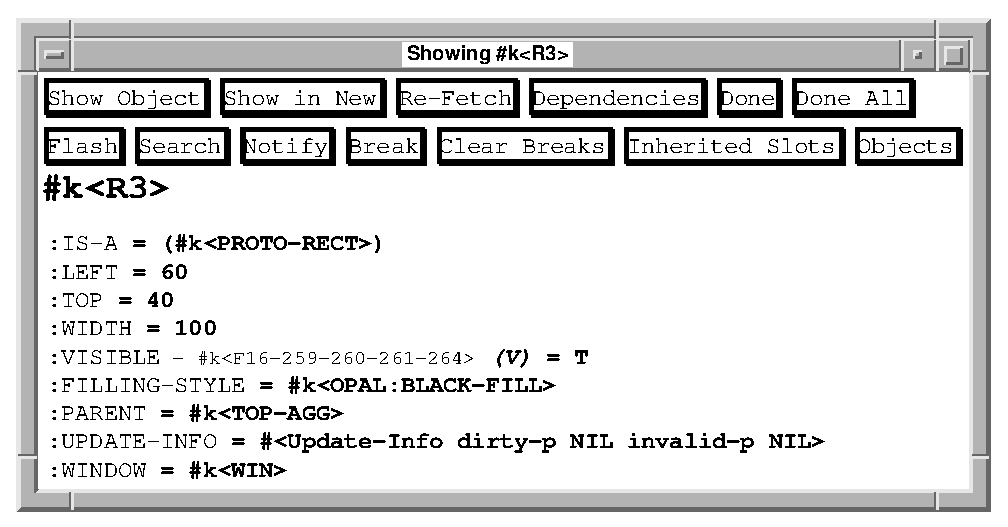
\epsfig{file=inspector.ps}
\end{latexonly}
  \htmladdimg{../gifs/inspector.gif}
\end{center}
\caption{The Inspector displaying the slots and values of rectangle R3.}
\tag{inspector}
%\bar{}
\end{figure}

The local slots and values for R3 are shown in the Inspector window.
Inherited slots are not shown, like \pr{:height} or \pr{:line-style} (assuming
that you did not set these slots yourself, installing local values in R3).
If you have a color screen, some slots are red, indicating that these slots
are public `parameters' of the object (we discuss parameters more in
section \ref{parameters}).

It is very easy to change properties of an object with the Inspector.  For
example, to change the \pr{:width} of R3 using the inspector, click the mouse
on the value of the \pr{:width} slot (which is 100 in figure \ref{inspector}).
Use standard Emacs commands to change the value of the slot to something
significantly different, like 20.  When you hit RETURN, the change will appear
instantly in R3.

To add a new local value to R3 -- that is, to override an inherited value with
a new local value -- you have to add an extra line to the Inspector window.
In our example, R3 does not have a local value for \pr{:height}, since its
value is inherited from the prototype PROTO-RECT.  To override this value,
click the cursor at the end of a line, and type \pr{{\tt\char`\^}j} to add a new line
to the display.  Now you can type `\pr{:height = 100}' and hit RETURN to
install the new slot/value pair.  The change should be reflected instantly
in R3.

You can bring up other Inspector windows by positioning the mouse over another
object and hitting HELP again, or you can select text that is already displayed
in the Inspector and using the `\pr{Show Object}' or `\pr{Show in New}'
buttons.  For example, to examine the \pr{opal:black-fill} object that is the
value of R3's \pr{:filling-style} slot, either click-and-drag or double-click
on the \pr{\#k<OPAL:BLACK-FILL>} value and press the `\pr{Show in New}' button.
The object will be displayed in a new window.

When you are finished with the Inspector, you can click on the `\pr{Done}' or
`\pr{Done All}' buttons to make the Inspector windows disappear.

Significantly more detail about the Inspector is included in the Debugging
Manual, including how to explore the Prototype/Instance hierarchy of objects,
and how to use the Inspector for debugging more compilcated examples.


\section{Parameters}
\label{parameters}

Most objects in Garnet have a list of {\it parameters}, which are stored in the
\pr{:parameters} slot.  This is a list of all customizable properties of
the object.  For example, \pr{gv opal:rectangle :parameter} yields:
%\vspace{.5 line}

\begin{programexample}
(:LEFT :TOP :WIDTH :HEIGHT :LINE-STYLE :FILLING-STYLE :DRAW-FUNCTION :VISIBLE)
\end{programexample}

These can be considered the `public' slots of \pr{opal:rectangle}, which can
be given customized values when instances are created.  If values are not
supplied for these slots when instances are created, the default values will
be inherited from the prototype object.

There are other slots that change when instances of \pr{opal:rectangle} are
added to a window, such as the \pr{:window} and \pr{:parent} slots, but these
slots are not intended to be set manually.  Since they are `read-only' slots,
they are not included in the \pr{:parameters} list.

Several tools in Garnet rely heavily on the \pr{:parameters} slot.
As discussed in section \ref{inspector-sec}, the Inspector displays the
parameter slots in red, so that they are easily identified.  The
\pr{gg:prop-sheet} gadget which is used in Gilt and Lapidary looks at the
\pr{:parameters} slot to determine which slots should be displayed for the
user to customize.  These objects are discussed thoroughly in later sections
of this reference manual.

The typical Garnet user will not have to worry much about the \pr{:parameters}
slot.  All of the slots that are in the list are documented in this manual,
so it is really just another way to access the same information about
properties of objects.  For details on defining \pr{:parameters} slots for
your own objects, see the KR Manual.  Unless you are defining your own
list for a special object, the \pr{:parameters} slot should be considered
read-only.


\section{Destroying Objects}
\label{destroying}

Before moving on to the next section, destroy the window so that it
does not interfere with future examples in this tutorial.  Type the
following line.

\begin{programexample}
(opal:destroy WIN)
\end{programexample}
				
Destroying the window will also destroy all of the objects that were
added to its aggregate.  We can no longer manipulate R1, R2, and R3,
since they were destroyed by the previous call.  However, the
PROTO-RECT was never added to the top-level aggregate, and it was not
destroyed.  You could destroy this object now with a \pr{destroy}
call, but we will be using this object again in Section
\ref{destroying}.  So, leave the object residing in memory for now.

When an object is destroyed, its variable name becomes unbound and the
memory space that was allocated to the object is freed.  You can
\pr{destroy} any object, including windows.  If you destroy a window,
all objects inside of it are automatically destroyed.  Similarly, if
you destroy an aggregate, all objects in it are destroyed.  When you
destroy a graphical object (like a line or a circle), it is
automatically removed from any aggregate it might be in and erased
from the screen.

If a prototype object is destroyed (i.e., an object that has had
instances created from it), then all of the instances of that object
will be recursively destroyed.

Occasionally in the course of developing a program, you may (either
accidentally or intentionally) define a new object which happens to
have the same name as an old object.  When the new object is created,
its variable name is set to the new object, and the old object by the
same name is destroyed.  Also, all of the instances of the old object
are recursively destroyed.

For example, in Section \ref{prototypes} above, we created the object
PROTO-RECT, which still exists in memory.  If we now enter the
following new schema definition for an object by the same name, then
the old PROTO-RECT will be destroyed.

\begin{programexample}
(create-instance 'PROTO-RECT opal:rectangle)
\end{programexample}

When the new schema is entered, a warning is given that the old object
is being destroyed.  You can safely ignore this message, assuming that
you intended to override the definition of the old schema.


\section{Unnamed Objects}
\label{unnamed-objects}

Sometimes you will want to create objects that do not have a
particular name.  For example, you may want to write a function that
returns a rectangle, but it will be called repeatedly and should not destroy
previous instances with new ones.  In this case, you should return an
unnamed rectangle from the function which can be used just like the
named objects we have created earlier in this tutorial.

As an example, the following code creates an
unnamed object and internally generates a unique variable name for it.
Instead of supplying a quoted name to \pr{create-instance}, we give it
the value NIL.

\begin{programexample}
(create-instance NIL opal:rectangle
   (:left 10) (:top 10) (:width 75) (:height 50))
\end{programexample}

When you enter this schema definition, the \pr{create-instance} call
will return the generated internal name of the rectangle -- something like
\pr{RECTANGLE-123}.  This name has a unique number as a
suffix that prevents it from being confused with other rectangles in
Garnet.  You can now use the generated name to refer to the object.

\begin{programexample}
(gv RECTANGLE-123 :top)  {\it ; Replace this name with the name of your rectangle.}
\end{programexample}

Usually it is convenient to assign an unnamed object to a local
variable.  The following line creates a circle and assigns it to the
new variable MY-CIRCLE.

\begin{programexample}
(setf MY-CIRCLE (create-instance NIL opal:circle))
\end{programexample}

Now MY-CIRCLE will have the generated circle as its value.  If the
same line were entered again, the old circle would not be destroyed,
but the variable MY-CIRCLE would still point to a new one.  This can
be useful inside a function that uses a \pr{let} clause -- every time
the \pr{let} is executed, new objects are assigned to the local
variables, but the old objects still remain in memory and are not
destroyed. Section \ref{function} contains an example of how unnamed
objects might be used in a function.


\chapter{An Overview of the Objects}

\section{Lines, Rectangles, and Circles}

The Opal package provides different graphical shapes
including circles, rectangles, roundtangles, and lines.  There are
also several different kinds of text, and some special objects like
bitmaps and arrowheads.  Each graphical object has special slots that
determine its appearance, which are documented in the Opal manual.
(For example, the line uses the slots \pr{:x1}, \pr{:y1}, \pr{:x2},
and \pr{:y2}.)
See the section  `Specific Graphical Objects' in the Opal manual for
details of how each object works.  Examples of creating instances of
graphical objects appear throughout this tutorial.


\section{Aggregates}
\label{aggregates}

In order to put a large number of objects into a window, we might
create all of the objects and then add them, one at a time, to the
window.  However, this is usually not how
we organize the objects conceptually.  For example, if we were to
create a sophisticated interface with a scroll bar, several buttons,
and labels for the buttons, we would not want to add each rectangle in
the scroll bar and the buttons individually.  Instead, we would think
of creating the scroll bar from its composite rectangles, then
creating the buttons along with their labels, and then adding the
scroll bar assembly and the button assembly to the window.

Grouping objects together like this is the function of the \pr{aggregate}
object.  Any graphical object can be a component of an aggregate - lines,
circles, rectangles, and even other aggregates.  Usually all of the
components of an aggregate are related in some way, like they are all
parts of the same button.

Two other objects, the \pr{aggregadget} and the
\pr{aggrelist}, are also used to group objects, and usually appear more
often in Garnet programs.  \pr{Aggregadgets} and \pr{aggrelists} are
instances of \pr{aggregate}, and they have special features that make
them very useful in creating objects.  These objects will be discussed
further in Section \ref{aggregadgets}.

The top-level object in a window is always an aggregate.  This
aggregate contains all of the objects in that window.
Therefore, for an object to appear in a window it either has to be a
component of the top-level aggregate, or it has to be a component of
another aggregate which, at the top of its aggregate hierarchy, is a
component of the top-level aggregate.

When aggregates have other aggregates as components, an aggregate hierarchy
is formed.  This hierarchy describes the way that objects are grouped together.
Figure \ref{v-scroll-hierarchy} shows how the objects that comprise a
vertical scroll bar might be conceptually organized.

% \begin{group}
\begin{figure}
%\bar{}
\begin{center}
%\graphic{Postscript=`tutorial/v-scroll-hierarchy.ps',boundingbox=File,magnify=.75}
\begin{makeimage}
\end{makeimage}
\begin{latexonly}
\epsfig{file=v-scroll-hierarchy.ps}
\end{latexonly}
    \htmladdimg{../gifs/v-scroll-hierarchy.gif}
                 \end{center}
\caption{One possible hierarchy for the objects that make up a scroll bar.}
\tag{v-scroll-hierarchy}
%\bar{}
\end{figure}
% \end{group}

In the scroll bar hierarchy, all of the leaves correspond to shapes
that appear in the scroll bar.  The leaves are always Opal graphic
primitives, like rectangles and text.  The nodes \pr{top-trill-box} and
\pr{bottom-trill-box} are both aggregates, each with two components.
And, of course, the top-level \pr{scroll-bar} node is an aggregate.

This aggregate hierarchy should not be confused with the inheritance
hierarchy that was discussed earlier.  Components of an aggregate do
not inherit values from their parents.  Instead, relationships among
aggregates and components must be explicitly defined using
constraints, a concept which will be discussed shortly in this tutorial.

When an object is added to an aggregate, its \pr{:parent} slot is set
to point to that aggregate.  Therefore, in Figure \ref{v-scroll-hierarchy},
the \pr{:parent} of the \pr{bottom-trill-box} is the \pr{scroll-bar}
aggregate.  This \pr{:parent} slot is called a {\it pointer} slot because
its value is another Garnet object.  Pointer slots are discussed
further in section \ref{aggregadgets}.

The functions \pr{add-component}, \pr{remove-component},
and \pr{move-component} are used to manipulate the components of an
aggregate.  Descriptions of these and other functions for components
may be found in the `Aggregate Objects' section of the Opal manual.


\section{Aggregadgets, Aggrelists, and Aggregraphs}
\label{aggregadgets}

Aggregadgets and aggrelists are types of aggregates.  With these
objects, an aggregate and its components can basically be defined
simultaneously.  In aggregadgets, all the components are defined
with a list in the \pr{:parts} slot.  In an aggrelist, a single object
is defined to be an `item-prototype', and the aggrelist automatically
generates several instances of that object to make its components.
The aggregraph is a type of aggregadget, where all the components are
nodes and arcs that make up a graph.  Figures \ref{opalInheritance}
and \ref{v-scroll-hierarchy} were created using Garnet aggregraphs.
For several examples and a complete discussion of how to use
aggregraphs, see the Aggregadgets, Aggrelists, and Aggregraphs
Reference Manual.


\subsection{Aggregadgets}

When you create an aggregadget, you may list all of the objects that
you want as components of the aggregadget in the \pr{:parts} slot.
The list is specified using the standard Lisp backquote macro, and
there are usually many function calls and objects inside the list that
must be evaluated with a comma.  As an example of an aggregadget, we
will analyze the following schema definition, but it is not necessary
to type it in.  This code contains a few references that have not been
discussed in this tutorial yet, but it serves the purpose of giving us
a plain aggregadget to study.

\begin{programexample}
(create-instance 'AGG opal:aggregadget
   (:left 10) (:top 20)
   (:parts
    `((:my-circle ,opal:circle
                  (:left 60) (:top 70)
                  (:width 100) (:height 100)
                  (:line-style ,opal:dashed-line))
      (:my-rect ,opal:rectangle
                (:left ,(o-formula (gvl :parent :left)))
                (:top ,(o-formula (gvl :parent :top)))
                (:width 80) (:height 40)
                (:filling-style ,opal:black-fill)
                (:line-style NIL)))))
\end{programexample}

The \pr{:parts} slot in the AGG object contains
a list of lists, with each internal list being a definition of a component.
The components of AGG will be a circle and a rectangle, to which we
have given the arbitrary names \pr{:my-circle} and \pr{:my-rect}.
These names, which are preceded by a colon, will be the names of new
slots in the aggregadget.  That is, two {\it pointer} slots will be
created in AGG, named \pr{:my-circle} and \pr{:my-rect}, which will
have the circle and rectangle objects as their values.  We say these are
pointer slots because they point to other objects.

Other pointer slots which are automatically created are the
\pr{:parent} slots of both the circle and the rectangle.  Since these
objects are being added as components to the aggregadget, their
\pr{:parent} slots are set as with aggregates.  Thus, a two-way path
of communication is established between the aggregadget and each of
its components -- the \pr{:parent} slot points up, and the
\pr{:my-circle} slot points down.

Notice that the \pr{:parts} list is backquoted
(with a \pr{`} instead of a \pr{'}).  Using this backquote syntax, we can then
use commas to evaluate the names of objects inside the list.  The
references to be evaluated are the two graphical object prototypes (the
\pr{opal:circle} and the \pr{opal:rectangle}) and the graphical
qualities (\pr{opal:dashed-line} and \pr{opal:black-fill}).
Commas are also used to evaluate the \pr{o-formula} calls, which
establish constraints among objects (constraints are discussed
in Chapter \ref{constraints}).  If the commas were not present inside
the \pr{:parts} list, then the names of all the Garnet objects would not be
dereferenced, and they would be treated as mere atoms, not objects.
Similarly, the calls to \pr{o-formula} would appear as simple quoted
lists instead of function calls.

An important difference between aggregates and aggregadgets is that
when you create an instance of an aggregadget, the instance will
automatically have components that match those in the prototype.  That
is, if we created an instance of AGG, called AGG-INSTANCE, then
AGG-INSTANCE would automatically have a circle and rectangle component
just like AGG.  In contrast, when you create an instance of an
aggregate, the components are not automatically generated, and you
would have to create and add them to the instance manually.

Other examples of aggregadget definitions
can be found in sections \ref{aggregadget-ex} and \ref{big-example} in
this tutorial.

\subsection{Aggrelists}

An aggrelist allows you to create and easily arrange objects into a
nicely formatted graphical list.  The motivation for aggrelists comes
from the arrangement of groups of objects like button panels,
tic-marks, and menu choices, where all the components of an aggregate
are similar and should appear in a vertical or horizontal list.

In an aggrelist, a single item-prototype is defined, and then this
object is automatically copied several times to make the components of
the aggrelist.  The \pr{:left}, \pr{:top}, and other slots of the
components are automatically given values that will neatly lay out the
components in a list, so that the programmer does not have to do any
calculations for the positions of the objects.

As with aggregadgets, aggrelists
use the backquote syntax to define the item prototype.  There are many
customizable aspects of aggrelists, such as whether to orient the
components vertically or horizontally, the distance between each
object, etc.  Since there are so many customizable slots, please see
the Aggregadgets and Aggrelists Reference Manual for a discussion of
how to use aggrelists.  Section \ref{big-example} in this tutorial
includes an example of the definition of an aggrelist.


\section{Windows}

When we want to add an object to a window, what we really mean is that we
want to add the object to the window's top-level aggregate (or to an
aggregate at a lower level in that window's aggregate hierarchy).
Every window has one top-level aggregate, and all objects that appear
in the window are components in its aggregate hierarchy.

Any object must be added to a window in order for it to be shown on
the screen.  Additionally, a window must be updated before any changes
made to it (or the objects in it) will appear.  Windows are updated
when you explicitly issue a call to \pr{opal:update}, and they are
also continuously updated when interactors are running and changing
objects in the window (during the \pr{main-event-loop}, discussed in
Section \ref{interactors}).


\section{Gadgets}

The Garnet gadgets are a set of ready-made widgets that can be treated
as regular graphical objects.  They have slots that can be customized
with user-defined values, and are added to windows just like graphical
objects.  Generally, they are objects that are
commonly found in an interface including scroll bars, menus, buttons
and editable text fields.  In the Tour, you created instances of the
radio button panel and the vertical slider.  There are also more
sophisticated gadgets like scrolling windows, property sheets (to
allow quick editing of the slots of objects), and selection handles
(for moving and growing objects).

Most of the gadgets come in two versions -- one called the Garnet
Style, and one modeled after the OSF/Motif style.  Examples of how to
use the gadgets are found in demonstration programs at the end of each
of the gadget files, which can be executed by commands like
\pr{(garnet-gadgets:menu-go)}.  For detailed descriptions of all the
available gadgets, see the Gadgets Reference Manual.



\chapter{Constraints}
\label{constraints}

In the course of putting objects in a window, it is often desirable to
define relationships among the objects.  For example, you may want
the tops of several objects to be aligned, or you might want a set of
circles to have the same center, or you may want an object to change
color if it is selected.  Constraints are used in Garnet to define
these relationships among objects.

Although all the examples in this section use constraints on the
positions of objects, it should be clear that constraints can be
defined for filling styles, strings, or any other property of a Garnet
object.  Many examples of constraints can be found in other sections
of this tutorial.  Additionally, much of the KR Reference Manual is
devoted to the discussion of constraints among objects.  The sections
`Constraint Maintenance' and `Slot and Value Manipulation Functions'
should be of particular interest.


\section{Formulas}

A formula is an explicit definition of how to calculate the value for
a slot.  If we want to constrain the top of one object to be the same
as another, then we define a formula for the \pr{:top} slot of the dependent
object.  With constraints, the value of one slot always {\it depends} on
the value of one or more other slots, and we say the formula in that
slot has {\it dependencies} on the other slots.

An important point about constraints is that they are constantly
maintained by the system.  That is, they are evaluated once when they
are first created, and then they are continually {\it re-evaluated} when
any of their dependencies change.  Thus, if several objects depend on
the top of a certain rectangle, then all the objects will change
position whenever the rectangle is moved.

\begin{figure}
%\bar{}
\begin{center}
%\graphic{Postscript=`tutorial/align-top.ps',boundingbox=File,magnify=.75}
\begin{makeimage}
\end{makeimage}
\begin{latexonly}
\epsfig{file=align-top.ps}
\end{latexonly}
    \htmladdimg{../gifs/align-top.gif}
\end{center}
\caption{Three objects that are all aligned with the same top.  The
top of the gray rectangle is constrained to the white rectangle, and
the top of the black circle is constrained to the top of the gray rectangle.}
\tag{align-top}
%\bar{}
\end{figure}

As our first example of defining constraints among objects, we will
make the window in Figure \ref{align-top}.  Let's begin by creating
the white rectangle at an absolute position, and then create the other objects
relative to it.  Create the window and the first box with the
following code.

\begin{programexample}
(create-instance 'CONSTRAINTS-WIN inter:interactor-window      {\it ; Create the window}
   (:left 750)(:top 80)(:width 260)(:height 100))
(create-instance 'TOP-AGG opal:aggregate)                      {\it ; Create an aggregate}
(s-value CONSTRAINTS-WIN :aggregate TOP-AGG)                   {\it ; Assign the aggregate to the window}
(opal:update CONSTRAINTS-WIN)                                  {\it ; Make the window appear}

(create-instance 'WHITE-RECT opal:rectangle                    {\it ; Create a rectangle}
   (:left 20) (:top 30)
   (:width 60) (:height 40)
   (:filling-style opal:white-fill))
		
(opal:add-components TOP-AGG WHITE-RECT)                       {\it ; Add the rectangle to the window}
(opal:update CONSTRAINTS-WIN)                                  {\it ; Make changes in the window appear}
\end{programexample}

We are now ready to create the other objects that are aligned with
WHITE-RECT.  We could simply create another rectangle and a circle that
each have their top at 30, but this would lead to extra work if we ever
wanted to change the top of all the objects, since each object's
\pr{:top} slot would have to be changed individually.  If we instead
define a relationship that depends on the top of WHITE-RECT, then
whenever the top of WHITE-RECT changes, the top of the other objects
will automatically change, too.  Define the schema for the gray
rectangle as follows.

\begin{programexample}
(create-instance 'GRAY-RECT opal:rectangle
   (:left 110)
   (:top (o-formula (gv WHITE-RECT :top)))  {\it ; Constrain the top of this rectangle to the top of WHITE-RECT}
   (:width 60) (:height 40)
   (:filling-style opal:gray-fill))

(opal:add-components TOP-AGG GRAY-RECT)
(opal:update CONSTRAINTS-WIN)
\end{programexample}

You can see that without specifying an absolute position for the top
of the gray rectangle, we have constrained it to always have the same
top as the white rectangle.  The formula in the \pr{:top} slot of
the gray rectangle was defined using the functions \pr{o-formula} and
\pr{gv}.  The \pr{o-formula} function is used to declare that an
expression is a constraint.  When \pr{gv} is used inside a formula,
it causes a dependency to be established on the referenced slot, so that
the formula will be reevaluated when the value in the referenced slot
changes.  \footnote{There is another function called \pr{g-value}
that is similar
to \pr{gv}, except that it never causes dependencies to be established.
Older versions of Garnet required that \pr{gv} only be used inside
formulas, and \pr{g-value} to be used ouside.  The \pr{gv} function has
since been enhanced so that it can be used everywhere.  It would be
unusual to ever need to use \pr{g-value}.}

To see if our constraint is working, try changing the
top of the white rectangle with the following instructions and notice
how the gray rectangle moves with it.  Try setting the top to other
values, if you wish.

\begin{programexample}
(s-value WHITE-RECT :top 50)
(opal:update CONSTRAINTS-WIN)
\end{programexample}

The important thing to notice is that the value of the \pr{:top} slot
of GRAY-RECT changes as the top of the WHITE-RECT changes.  This shows
that the formula in GRAY-RECT is being re-evaluated whenever its
depended values change.

Now we are ready to add the black circle to the window.  We have a
choice of whether to constrain the top of the circle to the white
rectangle or the gray rectangle.  Since we are going to be examining
these objects closely in the next few paragraphs, let's constrain the
circle to the gray rectangle, resulting in an indirect relationship with
the white one.  Define the black circle with the following code.

\begin{programexample}
(create-instance 'BLACK-CIRCLE opal:circle
   (:left 200)
   (:top (o-formula (gv GRAY-RECT :top)))
   (:width 40) (:height 40)
   (:filling-style opal:black-fill))

(opal:add-components TOP-AGG BLACK-CIRCLE)
(opal:update CONSTRAINTS-WIN)
\end{programexample}

At this point, you may want to set the \pr{:top} of the white
rectangle again just to see if the black circle follows along with
the gray rectangle.


\section{Cached Values}

An interesting question might have occurred to
you -- what happens if you set the \pr{:top} of the gray rectangle now?
Setting the value of a slot which already has a formula in it does {\it not}
destroy the existing constraint.  However, it does override the
current {\it cached} value of the formula.  Try setting the \pr{:top} of
the gray rectangle now.

\begin{programexample}
(s-value WHITE-RECT :top 30)  {\it ; Return everything to its original position}
(opal:update CONSTRAINTS-WIN)

(s-value GRAY-RECT :top 40)
(opal:update CONSTRAINTS-WIN)
\end{programexample}

The position of WHITE-RECT will remain unchanged, since it was defined with
an absolute position.  However, the new value that we gave for the top
of the gray rectangle has repositioned GRAY-RECT and BLACK-CIRCLE.
Previously, the formula in the \pr{:top} slot of GRAY-RECT had
correctly computed its own top, getting the value from the \pr{:top}
slot of WHITE-RECT.  Now, however, we replaced that cached value
with our absolute value of 40.

To show that the formula is still alive and well in the \pr{:top} slot
of GRAY-RECT, try setting the \pr{:top} slot of WHITE-RECT again.

\begin{programexample}
(s-value WHITE-RECT :top 10)
(opal:update CONSTRAINTS-WIN)
\end{programexample}

Since the top of GRAY-RECT depends on WHITE-RECT, its formula will be
recomputed whenever the top of WHITE-RECT changes.  There is now a new
cached value for the \pr{:top} of GRAY-RECT, a result of re-evaluating
the formula.


\section{Formulas and s-value}

It is important to distinguish the behavior of \pr{s-value} when it is
used on a slot with a formula in it, versus using it on a slot with an
absolute value in it (like the number 5).  Setting the value of a slot that
{\it already} has a formula in it will not destroy the old formula.
Instead, only the cached value of the formula is changed, and the
formula will be re-evaluated if any of its dependencies change.

On the other hand, \pr{s-value} will replace one absolute value with
another absolute value, and the old value will never appear again.
That is, if an object was created with some particular absolute value for a
slot, and we changed that slot with \pr{s-value}, then the new value
will be permanent until the slot is explicitly set again with \pr{s-value}.

The one exception to the above rules is when the new value is a
formula itself.  Using \pr{s-value} to set a new formula will always
obliterate what was previously in the slot, whether it was an absolute
value or a formula.


\section{Using the :obj-over Slot}
\label{obj-over-slot}

When designing an interface, you may want a box to be drawn
around an object to show that it is selected.  In the usual case, you
will want to define only one box that will be drawn around different
objects, and it would be nice if the box changed size when it was over
objects of different size.  The traditional Garnet approach to this
problem is to use constraints in the dimension slots of the selection
box that depend on the dimensions of the object it is over.

\begin{figure}
%\bar{}
\begin{center}
%\graphic{Postscript=`tutorial/obj-over.ps',boundingbox=File, magnify=.75}
\begin{makeimage}
\end{makeimage}
\begin{latexonly}
\epsfig{file=obj-over.ps}
\end{latexonly}
    \htmladdimg{../gifs/obj-over.gif}
\end{center}
\caption{A selection box drawn around an object.}
\tag{obj-over}
%\bar{}
\end{figure}

In the traditional approach, we use the slot \pr{:obj-over} in the
selection box to specify which object the selection box should be
drawn around.  The \pr{:obj-over} slot is a pointer slot, since it
contains an object as its value (pointer slots were discussed in
section \ref{aggregadgets}).  Then, we define formulas for the
dimensions of the selection box which depend on the \pr{:obj-over}
slot.  The formulas in the following schema definition should be clear.

\begin{programexample}
(create-instance 'SEL-BOX opal:rectangle
   (:obj-over GRAY-RECT)  {\it ; A pointer slot}
   (:left (o-formula (- (gvl :obj-over :left) 10)))
   (:top (o-formula (- (gvl :obj-over :top) 10)))
   (:width (o-formula (+ 20 (gvl :obj-over :width))))
   (:height (o-formula (+ 20 (gvl :obj-over :height))))
   (:line-style opal:line-4))  {\it ; A line with a thickness of 4 pixels}
		
(opal:add-components TOP-AGG SEL-BOX)
(opal:update CONSTRAINTS-WIN)
\end{programexample}

Now if you set the \pr{:obj-over} slot of the selection box to be a
different object, the position and dimensions of SEL-BOX will change
according to the object.

\begin{programexample}
(s-value SEL-BOX :obj-over BLACK-CIRCLE)
(opal:update CONSTRAINTS-WIN)
\end{programexample}

You may have noticed that we performed computations in the formulas
above, instead of just using values directly as in the GRAY-RECT and
BLACK-CIRCLE objects.  In fact, formulas can contain any lisp
expression.  Also, the formulas above use the function \pr{gvl}
instead of \pr{gv}, which was used earlier.  We use \pr{gvl} here
because we are referencing a slot, \pr{:obj-over}, in the same schema
as the formula.  Previously, we used \pr{gv} to look at a slot in a
different object.

Another point of interest in these formulas is the use of indirect
references.  In the \pr{:left} formula above, the pointer slot \pr{:obj-over}
is referenced, and then its \pr{:left} slot is referenced, in turn.
It is important to distinguish between this case and the case where
a value is stored in the same object as the formula, as in the
following example.

Suppose we want the selection box to become invisible if no object is
currently selected.  Using \pr{s-value}, we can set the \pr{:visible}
slot of SEL-BOX to have a formula which will cause the box to
disappear when its current selection is NIL.  (We could have also
defined this formula in the \pr{create-instance} call.)

\begin{programexample}
(s-value SEL-BOX :visible (o-formula (gvl :obj-over)))
\end{programexample}

Clearly, if \pr{:obj-over} is set to NIL, then the value in the
\pr{:visible} slot will also become NIL, and the box will become
invisible.  When \pr{:obj-over} is again set to be some object, then
the \pr{:visible} slot will have a non-NIL value, and the box will
appear in the appropriate position.  Previously, if we had set
\pr{:obj-over} to NIL, then updating the window would have caused an
error when the formulas tried to access the \pr{:left}, \pr{:top},
\pr{:width}, and \pr{:height} of the non-existent selected object.

We are finished with the objects from this section, but the next
section will continue to use the same window.  So, to remove the old
objects from the window, use the function \pr{remove-components}.

\begin{programexample}
(opal:remove-components TOP-AGG WHITE-RECT GRAY-RECT BLACK-CIRCLE SEL-BOX)
(opal:update CONSTRAINTS-WIN)
\end{programexample}


\section{Constraints in Aggregadgets}
\label{aggregadget-ex}

As mentioned in section \ref{aggregates}, the \pr{:parent} slot of a
component is automatically set to its parent aggregate when it is
attached.  Since aggregadgets are instances of aggregates, all of the
components defined in an aggregadget have their \pr{:parent} slot set
in this way.  In this section, we will examine how this slot can be
used to communicate between components of an aggregadget.

% \vspace{1 line}
%\begin{group}
The aggregadget we will use in this example will make the picture of
concentric circles in Figure \ref{concentric-circles}.  Suppose that
we want to be able to change the size and position of the circles
easily, and that this should be done by setting as few slots as
possible.
% \end{group}
% \vspace{.5 line}

\begin{figure}
%\bar{}
\begin{center}
% graphic{Postscript=`tutorial/con-circles.ps',boundingbox=File}
\begin{makeimage}
\end{makeimage}
\begin{latexonly}
\epsfig{file=con-circles.ps}
\end{latexonly}
    \htmladdimg{../gifs/con-circles.gif}
\end{center}
\caption{An aggregadget with three circles as components.}
\tag{concentric-circles}
%\bar{}
\end{figure}

From the picture, we see that the dimensions of the black circle are
the same as the dimensions of the entire group of objects.  That is,
if a bounding box were drawn around the black circle, all the other
objects would be inside the bounding box, too.
Therefore, it will be helpful to put slots for the size and position
of this circle in the top-level aggregadget, and have all the circles
reference these top-level values through formulas.

To start, let's create an aggregadget with only one component -- the
black circle -- and then redefine the aggregadget with the other
components later.  The following code creates this one-component
aggregate.

\begin{programexample}
(create-instance 'CON-CIRCLES opal:aggregadget
   (:left 20) (:top 20)
   (:width 100)
   (:height (o-formula (gvl :width)))
   (:parts
    `((:black-circle ,opal:circle
                     (:left ,(o-formula (gvl :parent :left)))
                     (:top ,(o-formula (gvl :parent :top)))
                     (:width ,(o-formula (gvl :parent :width)))
                     (:height ,(o-formula (gvl :width)))
                     (:filling-style ,opal:black-fill)))))

(opal:add-component TOP-AGG CON-CIRCLES)
(opal:update CONSTRAINTS-WIN)
\end{programexample}

All those commas are needed because we want the Opal objects and the
calls to \pr{o-formula} to be evaluated inside the backquoted list.
If the commas were not present, then those forms would become inert
atoms and lists instead of objects and function calls.

The black circle in the aggregadget gets its position and
dimensions from the top-level slots in CON-CIRCLES.  The communication
link used here is the \pr{:parent} slot, which points from the
component to the aggregadget.  The function
\pr{gvl} is used in the formulas for the black circle because the
\pr{:parent} slot is in the same object as the formulas.  Notice that
the black circle does {\it not} `inherit' any values from its parent.
Creating components in an aggregadget sets up an {\it aggregate}
hierarchy, where values travel back-and-forth over constraints,
not inheritance links.  If you want a component to depend on values in
its parent, you have to define constraints.

The other components of CON-CIRCLES will be defined analogously, but with
a little more computation in the formulas to get them to line up properly.
Before typing in the new definition of CON-CIRCLES, remove the old
aggregadget from the window with the following instruction.

\begin{programexample}
(opal:remove-components TOP-AGG CON-CIRCLES)
(opal:update CONSTRAINTS-WIN)
\end{programexample}

And now we are ready to redefine CON-CIRCLES again, this time with an
extra top-level slot to reduce redundant calculations, and of course
with the other two circles.

\begin{programexample}
(create-instance 'CON-CIRCLES opal:aggregadget
   (:left 20) (:top 20)
   (:width 100)
   (:height (o-formula (gvl :width)))
   (:radius/3 (o-formula (round (gvl :width) 6)))
   (:parts
    `((:black-circle ,opal:circle
                     (:left ,(o-formula (gvl :parent :left)))
                     (:top ,(o-formula (gvl :parent :top)))
                     (:width ,(o-formula (gvl :parent :width)))
                     (:height ,(o-formula (gvl :width)))
                     (:filling-style ,opal:black-fill))
      (:gray-circle ,opal:circle
                    (:left ,(o-formula (+ (gvl :parent :left)
					  (gvl :parent :radius/3))))
                    (:top ,(o-formula (+ (gvl :parent :top)
					 (gvl :parent :radius/3))))
                    (:width ,(o-formula (- (gvl :parent :width)
					   (* 2 (gvl :parent :radius/3)))))
                    (:height ,(o-formula (gvl :width)))
                    (:filling-style ,opal:gray-fill))
      (:white-circle ,opal:circle
                     (:left ,(o-formula (+ (gvl :parent :gray-circle :left)
					   (gvl :parent :radius/3))))
                     (:top ,(o-formula (+ (gvl :parent :gray-circle :top)
					  (gvl :parent :radius/3))))
                     (:width ,(o-formula (- (gvl :parent :gray-circle :width)
					    (* 2 (gvl :parent :radius/3)))))
                     (:height ,(o-formula (gvl :width)))
                     (:filling-style ,opal:white-fill)))))

(opal:add-components TOP-AGG CON-CIRCLES)
(opal:update CONSTRAINTS-WIN)
\end{programexample}

The gray circle gets its size and position from the top-level slots
just like the black circle, only it is one-third the size.  The white circle
is the most interesting case, where it gets its position and
dimensions from the gray circle.  Not only does the white circle
communicate with the aggregadget through the \pr{:parent} slot, but it
also uses the slot \pr{:gray-circle} which was automatically created
in the aggregadget (see section \ref{aggregadgets}).  Thus, the
formulas in the white circle trace up the aggregate hierarchy to the
parent aggregadget, and then back down into another component.

To examine these pointer slots more closely, try executing the
following line.

\begin{programexample}
(gv CON-CIRCLES :white-circle)
\end{programexample}

The value returned by this \pr{gv} call is the internally
generated name of the white circle.  This name was generated with a
unique suffix number so that it will not be confused with some other
white circle in Garnet (see Section \ref{unnamed-objects}).  You can
also look at slots of the components directly, by adding slot names to
the end of the \pr{gv} call, like

\begin{programexample}
(gv CON-CIRCLES :white-circle :top)
\end{programexample}

or even

\begin{programexample}
(gv CON-CIRCLES :white-circle :parent)
\end{programexample}

This is the end of the section regarding constraints.  Destroy the window
we have been using to keep it from interfering with future examples in
the tutorial.

\begin{programexample}
(opal:destroy CONSTRAINTS-WIN)
\end{programexample}



\chapter{Interactors}
\label{interactors}

Interactors are used to communicate with the mouse and keyboard.
Sometimes you may just want a function to be executed when the mouse
is clicked, but often you will want changes to occur in the graphics
depending on the actions of the mouse.  Examples include moving
objects around with the mouse, editing text with the mouse and
keyboard, and selecting an object from a given set.

The fundamental way that the interactors communicate with graphical
objects is that they set slots in the objects in response to mouse
movements and keyboard key strokes.  That is, they generate side
effects in the objects that they operate on.  For example, some interactors
set the \pr{:selected} and \pr{:interim-selected} slots to indicate which
object is currently being operated on.  When objects are defined with
formulas that depend on these special slots, the appearance of the
objects (i.e., the graphics of the interface) can change in response
to the mouse.

It is important to note that all of the gadgets come with their
interactors already defined.  Therefore, you do not need to create
interactors that change the gadgets.

In this section we will see some examples of how to change graphics in
conjunction with interactors.  Section \ref{trace-inter} describes how
to use an important debugging function for interactors called
\pr{trace-inter}.   Although this tutorial only gives examples of
using the \pr{button-interactor} and \pr{move-@{\tt\char`\|}grow-@{\tt\char`\|}interactor}, the
Interactors Manual discusses and provides examples for all six types
of Garnet interactors.


\section{Kinds of Interactors}

The design of the interactors is based on the observation that there
are only a few kinds of behaviors that are typically used in graphical
user interfaces.  Currently, Garnet supports seven types of interactive
behavior, which allows a wide variety of user actions in an interface.
Below is a list of the available interactors, which are described in
detail in the Interactors Manual.

\begin{description}
\item[] \pr{Menu-Interactor} - For selecting one or more choices from a set of
items.  Useful in menus, etc., where the mouse may be held down and
dragged while moving over the items to be selected.

\item[] \pr{Button-Interactor} - For selecting one or more choices from a set
of items.  Useful in single buttons and panels of buttons where the
mouse can only select one item per mouse click.

\item[] \pr{Move-Grow-Interactor} - For moving and changing the size of an
object.  Useful in scroll bars and graphics editors.

\item[] \pr{Two-Point-Interactor} - For obtaining one or two points in a
window from the user.  Useful in specifying the size and position of a
new object to be created.

\item[] \pr{Angle-Interactor} - For getting the angle that the mouse moves
around a point.  Useful in circular gauges or for `stirring motions'.

\item[] \pr{Text-Interactor} - For editing strings.  Most useful for small
strings, since Garnet does not support complicated word-processing
applications.

\item[] \pr{Gesture-Interactor} - For recognizing gestures drawn by the user
(e.g., the user draws a rough shape that Garnet recognizes as a square).

\item[] \pr{Animator-Interactor} - For executing a function at regular intervals,
allowing rapid updating of graphics.
\end{description}

There are also several interactors that work with the \pr{multifont-text}
object.  This object and its associated interactors are discussed in
the Opal manual.


\section{The Button Interactor}

In this example, we will perform an elementary operation with an
interactor.  We will create a window with a white rectangle inside,
and then create an interactor that will make it change colors when
the mouse is clicked inside of it.  First, create the window with the
white rectangle.

\begin{programexample}
(create-instance 'INTER-WIN inter:interactor-window
   (:left 750)(:top 80)(:width 250)(:height 250))
(create-instance 'TOP-AGG opal:aggregate)
(s-value INTER-WIN :aggregate TOP-AGG)
(opal:update INTER-WIN)

(create-instance 'CHANGING-RECT opal:rectangle
   (:left 20) (:top 30)
   (:width 60) (:height 40)
   (:filling-style (o-formula (if (gvl :selected)
				  opal:black-fill
				  opal:white-fill)))
   (:selected NIL))  {\it ; Set by the interactor}

(opal:add-components TOP-AGG CHANGING-RECT)
(opal:update INTER-WIN)
\end{programexample}

From the definition of the \pr{:filling-style} formula, you can see
that if the \pr{:selected} slot in CHANGING-RECT were to be set to be
non-NIL, then its color would turn to black.  Conveniently, setting the
\pr{:selected} slot is one of the side effects of the
\pr{button-interactor}. The following code defines an interactor which
will set the \pr{:selected} slot of CHANGING-RECT, which will cause it
to change colors.

\begin{programexample}
(create-instance 'COLOR-INTER inter:button-interactor
   (:window INTER-WIN)
   (:start-where (list :in CHANGING-RECT))
   (:start-event :leftdown))

{\it ; Unless using CMU, Allegro, Lucid, LispWorks, or MCL}
\textit{; SBCL with thread support should work, too. }
(inter:main-event-loop)
{\it ; Hit F1 while the mouse is in the Garnet window to exit}
\end{programexample}

The \pr{main-event-loop} function causes Garnet to start paying
attention to events (like clicking the mouse) that trigger the interactors.
(A background process in CMU, Allegro, Lucid, LispWorks, and MCL always
pays attention to events.\footnote{As of Jan 2006, we believe that
  background threading also works with threaded SBCL, but this has not
been thoroughly tested.})
Now you can click on the rectangle
repeatedly and it will change from white to black, and back again.
From this observation, and knowing how we defined the
\pr{:filling-style} of CHANGING-RECT, you can conclude that the
\pr{button-interactor} is setting (and clearing) the \pr{:selected}
slot of the object.  This is one of the functions of the
\pr{button-interactor}.
When you are ready to resume typing in the Lisp process, you have to
hit the F1 key while the mouse is in the Garnet window to get a new
prompt.  (You may execute the \pr{main-event-loop} call again at any
Lisp prompt.)

\begin{figure}
%\bar{}
\begin{center}
% graphic{Postscript=`tutorial/inter-white.ps',boundingbox=File}
\begin{makeimage}
\end{makeimage}
\begin{latexonly}
\epsfig{file=inter-white.ps}  % graphic{Postscript=`tutorial/inter-black.ps',boundingbox=File}
\end{latexonly}
    \htmladdimg{../gifs/inter-white.gif}
\begin{latexonly}
\epsfig{file=inter-black.ps}
\end{latexonly}
    \htmladdimg{../gifs/inter-black.gif}
\end{center}
\caption{The rectangle CHANGING-RECT when its \pr{:selected} slot is NIL
(the default), and when it is set to T by the interactor (when the
mouse is clicked over it).}
%\bar{}
\end{figure}


\section{A Feedback Object with the Button Interactor}
\label{button-feed}

The method we used in the previous section with the
\pr{button-interactor} involved setting the \pr{:selected} slot of the
selected object.  There is another way to use the button interactor
which involves using feedback objects.  A {\it feedback object} is some
object that indicates the currently selected object.  For example, it is
often desirable that the actual selected object not move or change
color, but rather that a separate object follow the mouse or appear
over the selection.

In an earlier example in section \ref{obj-over-slot}, we defined a
selection box which works just like a feedback object.  When the
\pr{:obj-over} slot of the selection box was set to the name of the
selected object, then the box appeared around the selected object.  In this
example, we will redefine the objects from that section and create an
interactor to work on them.

The following code is analogous to what was presented in section
\ref{obj-over-slot}, but here the three selectable objects are defined as
components in an aggregadget.  Type in the following aggregadget and
feedback object, and add them to the current window.  Notice that
because of the \pr{:visible} formula in FEEDBACK-RECT, that rectangle
will be invisible when the window is first updated.

\begin{programexample}
(create-instance 'AGG opal:aggregadget
   (:top 100)
   (:parts
    `((:white-rect ,opal:rectangle
                   (:left 20)
                   (:top ,(o-formula (gvl :parent :top)))
                   (:width 60)
                   (:height 40)
                   (:filling-style ,opal:white-fill))
      (:gray-rect ,opal:rectangle
                  (:left 110)
                  (:top ,(o-formula (gvl :parent :top)))
                  (:width 60)
                  (:height 40)
                  (:filling-style ,opal:gray-fill))
      (:black-circle ,opal:circle
                     (:left 200)
                     (:top ,(o-formula (gvl :parent :top)))
                     (:width 40)
                     (:height 40)
                     (:filling-style ,opal:black-fill)))))

(create-instance 'FEEDBACK-RECT opal:rectangle
   (:obj-over NIL)  {\it ; A pointer slot to be set by the interactor}
   (:visible (o-formula (gvl :obj-over)))
   (:left (o-formula (- (gvl :obj-over :left) 10)))
   (:top (o-formula (- (gvl :obj-over :top) 10)))
   (:width (o-formula (+ 20 (gvl :obj-over :width))))
   (:height (o-formula (+ 20 (gvl :obj-over :height))))
   (:line-style opal:line-4))

(opal:add-components TOP-AGG AGG FEEDBACK-RECT)
(opal:update INTER-WIN)
\end{programexample}

Notice that the \pr{:obj-over} slot of FEEDBACK-RECT is a pointer
slot, as usual.  When \pr{:obj-over} is set with the name of an
object, the FEEDBACK-RECT will appear over the object because of the
way we defined its position and dimension formulas.  In this example,
we will not set \pr{:obj-over} by hand, as we did previously.
Instead, we will create a \pr{button-interactor} to set the slot for us.

The following code defines an interactor which uses the FEEDBACK-RECT
to indicate which object is selected.  Since all of the selectable
objects are in the same aggregate, we can tell the interactor to start
whenever the mouse is clicked over any component of AGG.

\begin{programexample}
(create-instance 'SELECTOR inter:button-interactor
   (:window INTER-WIN)
   (:start-where (o-formula (list :element-of AGG)))  {\it ; Work on the components of AGG}
   (:final-feedback-obj FEEDBACK-RECT)
   (:how-set :toggle))

{\it ; Unless using CMU, Allegro, Lucid, LispWorks, or MCL} 
\textit{; ... or probably threaded SBCL}
(inter:main-event-loop)
{\it ; Hit F1 while the mouse is in the Garnet window to exit}
\end{programexample}

Now when you click on the objects, the feedback object will appear
over the selected object.  The reason is that the
\pr{button-interactor} sets the \pr{:obj-over} slot of the feedback
object.  Since the interactor is a toggling
interactor (according to its \pr{:how-set} slot), the \pr{:obj-over}
slot will be reset to NIL when the selected object is clicked on again.

If you entered the \pr{main-event-loop}, remember to hit the F1 key
before typing in the next example.


\section{The Move-Grow Interactor}

From the previous example, you can see that it is easy to change the
graphics in the window using the mouse.  We are now going to define several
more objects in the window and create an interactor to move them.

The side effect of the \pr{move-grow-interactor} is that it sets the
\pr{:box} slot of the selected object (as well as the feedback object,
if any) to be a list of four values -- the left, top, width, and
height of the object.  When formulas are defined in the \pr{:left},
\pr{:top}, \pr{:width}, and \pr{:height} slots which depend on
the \pr{:box} slot, then the position and dimensions of the
object will change whenever the \pr{:box} slot changes.

The idea goes like this:  Suppose the current value of the \pr{:box}
slot in a rectangle is '(0 0 40 40).  Since the \pr{:left} and
\pr{:top} slots are constrainted to the \pr{:box} slot, the rectangle
appears at the position (0,0).  To move the object, the user clicks
and drags on the rectangle until it is at position (50,50).  When the
user lets go, then the interactor automatically sets the \pr{:box}
slot to '(50 50 40 40).  Since the \pr{:box} slot has changed, the
formulas in the \pr{:left} and \pr{:top} slot are re-evaluated, and
the rectangle appears at the new position.

The following code creates a prototype circle and several instances of
it.  With a little study, it should be clear how the position and dimension
formulas work with respect to the \pr{:box} slot.  All of the circles
are then added to an aggregate, and this aggregate is added as a
component to the top-level aggregate.

\begin{programexample}
(create-instance 'MOVING-CIRCLE opal:circle
   (:box '(0 0 40 40))  {\it ; This slot will be set by the interactor}
   (:left (o-formula (first (gvl :box))))     {\it ; Get the first value in the list}
   (:top (o-formula (second (gvl :box))))
   (:width (o-formula (third (gvl :box))))
   (:height (o-formula (fourth (gvl :box)))))

(create-instance 'M1 MOVING-CIRCLE
   (:box '(120 30 40 40)))

(create-instance 'M2 MOVING-CIRCLE
   (:box '(30 100 60 60)))

(create-instance 'M3 MOVING-CIRCLE
   (:box '(120 100 80 80)))

(create-instance 'CIRCLE-AGG opal:aggregate)

(opal:add-components CIRCLE-AGG M1 M2 M3)		

(opal:add-components TOP-AGG CIRCLE-AGG)
(opal:update INTER-WIN)
\end{programexample}

If you want to try setting the \pr{:box} slot of any of these objects,
you will see how the position and dimension of each circle depend on
it.  Be sure you set the \pr{:box} slot to be a list of four positive
numbers, or an error will occur!

Now let's create an instance of the \pr{move-grow-interactor}, which
will cause the moving circles to change position.  The following
interactor works on all the components of the aggregate CIRCLE-AGG.
Remember to execute the \pr{inter:main-event-loop} call to start the
interactors working.

\begin{programexample}
(create-instance 'MG-INTER inter:move-grow-interactor
   (:window INTER-WIN)
   (:start-where (list :element-of CIRCLE-AGG)))    {\it ; Work on the components of CIRCLE-AGG}

{\it ; Unless using CMU, Allegro, Lucid, LispWorks, or MCL}
\textit{; ... or probably threaded SBCL}
(inter:main-event-loop)
{\it ; Hit F1 while the mouse is in the Garnet window to exit}
\end{programexample}

Now if you press and drag in any of the circles, they will follow the
mouse.  This is because the interactor sets the \pr{:box} slot of the
object that it is pressed over, and the \pr{:left} and \pr{:top} slots
of the objects depend on the \pr{:box} slot.

It is worth noting once again that the \pr{move-grow-interactor} does
{\it not} set the \pr{:left}, \pr{:top}, etc. slots of the selected
object.  It instead sets the {\it \pr{:box}} slot of the selected
object, and the user is required to define formulas that depend on the
\pr{:box} slot.


\section{A Feedback Object with the Move-Grow Interactor}

Now let's add a feedback object to the window that will work with the
moving circles.  In this case, the feedback object will appear
whenever we click on and try to drag a circle.  The mouse will
actually drag the feedback object, and then the real circle will jump
to the final position when the mouse is released.

Our feedback object will be a circle with a dashed line.  The
DASHED-CIRCLE object defined below will have two slots set by the
interactor.  The \pr{:box} slot will be set while the mouse is held
down and dragged, and the \pr{:obj-over} slot will be set to point to the
circle being dragged.  Given our MOVING-CIRCLE prototype, the feedback
object is easy to define.

\begin{programexample}
(create-instance 'DASHED-CIRCLE MOVING-CIRCLE
   {\it ; Inherit all the :left, :top, etc. formulas that depend on the :box slot.}
   (:obj-over NIL)  {\it ; Set by the interactor}
   (:visible (o-formula (gvl :obj-over)))
   (:line-style opal:dashed-line))

(opal:add-components TOP-AGG DASHED-CIRCLE)
\end{programexample}

The \pr{:visible} slot is set with a formula because we only want the
feedback object to be visible when it is being used with the
interactor.  Now, we will redefine the move-grow interactor to use
DASHED-CIRCLE as a feedback object.  (Redefining the MG-INTER will
destroy the old instance, so don't worry if a warning appears.)

\begin{programexample}
(create-instance 'MG-INTER inter:move-grow-interactor
   (:window INTER-WIN)
   (:start-where (list :element-of CIRCLE-AGG))
   (:feedback-obj DASHED-CIRCLE))
\end{programexample}

Now when you move the circles with the mouse, the feedback object will
follow the mouse, instead of the real circle following it directly.

Since we have finished this section on interactors, destroy the window
so that it does not interfere with the next example.  Type the
following line.

\begin{programexample}
(opal:destroy INTER-WIN)
\end{programexample}


\chapter{Programming}

\section{Creating a Panel of Text Buttons}
\label{big-example}

In this section, we will go through a comprehensive example that pulls
together all the concepts that have been discussed in this tutorial.
The final objective will be the panel of text buttons in Figure
\ref{textButtons}.  We will use an aggregadget to assemble a group
of objects into a single button, then use an aggrelist to make
multiple copies of the text button and organize them into a list for
the panel, and finally create a button interactor to manage the panel.


\subsection{The Limitations of Aggregates}

Before starting the aggregadget for this example, let's take a look at the use
of an aggregate.  This will help to demonstrate the usefulness of
aggregadgets.  First, create a window with a top-level aggregate and
update it:

\begin{programexample}
(create-instance 'BUTTON-WIN inter:interactor-window
   (:left 800)(:top 10)(:width 200)(:height 400))
(create-instance 'TOP-AGG opal:aggregate)
(s-value BUTTON-WIN :aggregate TOP-AGG)
(opal:update BUTTON-WIN)
\end{programexample}

The TOP-AGG aggregate is the top-level aggregate for the window.  If
we want any object to appear in the window, it will have to be added
to TOP-AGG, or added to an aggregate further below in TOP-AGG's
aggregate hierarchy.  We will keep TOP-AGG as the top-level aggregate
throughout this example, but we will be changing its components continually.

Now we can begin adding objects to TOP-AGG (throughout this discussion
you should periodically check Figure \ref{textButtons} to see why we
are creating particular objects).  Let's start by assembling a button.
We will first create a couple of rectangles that have a fixed position
so that we get the window in Figure \ref{twoRects}.  Since we
want the rectangles to have the same dimensions, we can make a
prototype object and then create two instances with appropriate
position values.

\begin{programexample}
(create-instance 'PROTO-RECT opal:rectangle
   (:width 100) (:height 50))

(create-instance 'R1 PROTO-RECT
   (:left 40) (:top 40)
   (:filling-style opal:black-fill))

(create-instance 'R2 PROTO-RECT
    (:left 20) (:top 20)
    (:filling-style opal:gray-fill))

(opal:add-components TOP-AGG R1 R2)
(opal:update BUTTON-WIN)
\end{programexample}

\begin{figure}
%\bar{}
\begin{center}
% graphic{Postscript=`tutorial/two-rects.ps',boundingbox=File,magnify=.75}
\begin{makeimage}
\end{makeimage}
\begin{latexonly}
\epsfig{file=two-rects.ps}
\end{latexonly}
    \htmladdimg{../gifs/two-rects.gif}
\end{center}
\caption{The two rectangles R1 and R2, which are instances of PROTO-RECT.}
\tag{twoRects}
%\bar{}
\end{figure}

Keeping in mind our goal of making a panel of text buttons, one
problem should be immediately clear.  In order to make several
buttons with this method, we will have to calculate the position of
every rectangle in the interface and explicitly create an object for
it.  This will be time consuming, to say the least, and motivates us
to investigate how constraints will help avoid tedious calculations.
So, as the first step in pursuing a more fruitful approach, let's
remove the rectangles from the window and move on to aggregadgets.
To remove the rectangles, execute:

\begin{programexample}
(opal:remove-components TOP-AGG R1 R2)
(opal:update BUTTON-WIN)
\end{programexample}


\subsection{Using an Aggregadget for the Text Button}

When we create an aggregadget, we essentially create an aggregate and
add the components (along with pointer slots) all at once.  Our task
is to build an aggregadget
with two rectangles as components which will look like Figure
\ref{twoRects}.  Since we already know what we want the
rectangles to look like in the window, putting a simple aggregadget
together using our previously defined R1 and R2 rectangles is
straightforward.  However, the key to avoiding tedious
calculations of the positions of our rectangles is to generalize the
code.  That is, we want the positions of our components to be formulas
rather than absolute numbers.

For the present, let's assume that we will always be giving absolute
numbers to our top-level aggregadget (but not its components).  The first
problem we want to address
is how to devise formulas for the positions of the rectangles.
By referring back to Figure \ref{twoRects},
we see that the entire aggregate has its upper-left
coordinate at one corner of the gray rectangle, and its lower-right
coordinate on the shadow.  Therefore, it is a reasonable design
decision to put the left and top of the gray rectangle at the left,
top corner of the aggregadget, and then put the shadow 20 pixels
further below and to the right.  The following code shows the
definition of our new BUTTON aggregadget with formulas defined for the
positions of the rectangle components.

\begin{programexample}
(create-instance 'BUTTON opal:aggregadget
   (:left 20) (:top 20)
   (:shadow-width 100) (:shadow-height 50)
   (:parts
    `((:shadow ,opal:rectangle
	       (:left ,(o-formula (+ 20 (gvl :parent :left))))
	       (:top ,(o-formula (+ 20 (gvl :parent :top))))
	       (:width ,(o-formula (gvl :parent :shadow-width)))
	       (:height ,(o-formula (gvl :parent :shadow-height)))
	       (:filling-style ,opal:black-fill))
      (:gray-rect ,opal:rectangle
		  (:left ,(o-formula (gvl :parent :left)))
		  (:top ,(o-formula (gvl :parent :top)))
		  (:width ,(o-formula (gvl :parent :shadow-width)))
		  (:height ,(o-formula (gvl :parent :shadow-height)))
		  (:filling-style ,opal:gray-fill)))))

(opal:add-components TOP-AGG BUTTON)
(opal:update BUTTON-WIN)
\end{programexample}

After studying the BUTTON schema for a moment, several features stand out.
First, there are two slots called \pr{:shadow-width} and
\pr{:shadow-height} defined in the top-level schema, which are used by
the width and height formulas of the component rectangles.  The
presence of these slots at the top-level will make it easier to change
the appearance of the button in the future -- if we want to make it
wider, we only need to change one slot, \pr{:shadow-width}, instead
of all the components' \pr{:width} slots.

Next, it should be clear that the formulas in the \pr{:left} and
\pr{:top} slots of the components will place the rectangles at the
appropriate positions relative to each other, with the shadow further
down and to the right.  Finally, it is important that the shadow comes
first in the order of defining the components.  Objects are drawn on
the screen in the order that they are added to an aggregate, so we
definitely want the gray rectangle to come after the shadow.

Notice that there is no `inheritance' going on in the BUTTON
aggregadget.  When we want a component to get a value from its parent,
we have to explicitly define a constraint that gets that value.

We have just finished the first step in creating a text button.
Although there is more code in the aggregadget example than in the
previous example with rectangles R1 and R2, the aggregadget code is
simple and flexible.  Also, almost all of the formulas that you will
write in the future will resemble those in this example.  The only
difference will be the names of the slots and the arithmetic that is
appropriate for the situation.

Now we are ready to add more objects to the button.  To do this, we will
not add objects to BUTTON while it is in the window.  Instead, we will
remove the old BUTTON aggregadget from the window and write a new one from
scratch.  Most of the code that we have already written will be reused,
however, and if you still have a copy of the previous example on your screen,
you will be able to cut-and-paste it.  So execute the command that
will remove the button from the top-level aggregate:

\begin{programexample}
(opal:remove-components TOP-AGG BUTTON)
(opal:update BUTTON-WIN)
\end{programexample}


\subsection{Defining Parts Using Prototypes}

Before constructing an aggregadget with additional components, let's
look at another way to define components in aggregadgets.  This method
will make it easier for us to develop the BUTTON aggregadget by
condensing some of the code and eliminating a lot of typing.

In the previous example, the components were instances of rectangles.
Another way to define components is to define them as prototypes
separate from the aggregadget, and then create instances of those
prototypes in the aggregadget \pr{:parts} slot.  The following code
comes from this alternate method for defining aggregadgets.

\begin{programexample}
(create-instance 'SHADOW-PROTO opal:rectangle
   (:left (o-formula (+ 20 (gvl :parent :left))))
   (:top (o-formula (+ 20 (gvl :parent :top))))
   (:width (o-formula (gvl :parent :shadow-width)))
   (:height (o-formula (gvl :parent :shadow-height)))
   (:filling-style opal:black-fill))

(create-instance 'GRAY-PROTO opal:rectangle
   (:left (o-formula (gvl :parent :left)))
   (:top (o-formula (gvl :parent :top)))
   (:width (o-formula (gvl :parent :shadow-width)))
   (:height (o-formula (gvl :parent :shadow-height)))
   (:filling-style opal:gray-fill))

(create-instance 'BUTTON opal:aggregadget
   (:left 20) (:top 20)
   (:shadow-width 100) (:shadow-height 50)
   (:string `Button')
   (:parts
    `((:shadow ,SHADOW-PROTO)
      (:gray-rect ,GRAY-PROTO))))

(opal:add-components TOP-AGG BUTTON)
(opal:update BUTTON-WIN)
\end{programexample}


Notice that this way of looking at aggregadgets is entirely consistent
with the previous aggregadget definition.  In the \pr{:parts} slot of
our new button, we have created instances just like before, but we
have not explicitly defined any slots in the components.  It does not matter
whether we set slots in the prototype objects or in the parts
definitions.  Using this abbreviation method for defining aggregadgets,
we can now avoid retyping the slot definitions for the old components
and move on to talking about new ones.

It should be noted that the SHADOW-PROTO and GRAY-PROTO rectangles can
not be added to a window by themselves.  If you were to try this, you
would get an error when Garnet tried to evaluate any of the formulas
that we defined.  This is because there is no \pr{:parent} for either
the SHADOW-PROTO or the GRAY-PROTO, which is clearly needed by the
formulas.  But when instances of these rectangles are added to the BUTTON
aggregadget, their \pr{:parent} slots are set to be the parent aggregadget.

As usual, remember to remove the current BUTTON from the window using
\pr{remove-components}.


\subsection{The Label of the Button}

Referring to Figure \ref{textButtons} again, we see that the text
button needs a white rectangle to be centered over the gray one, and text
should be centered inside the white rectangle.  We will want the string of
the text object to be a top level slot in the aggregadget so that we
can change it easily.  Thus, we need to place a constraint in the text
object to retrieve it (remember the text object does not `inherit' the
string from its parent just because it is a component).  Other than
that, the addition of the new
components to the BUTTON aggregadget is straightforward.  Using the
abbreviation method for defining aggregadgets, we get the following code
(the components SHADOW-PROTO and GRAY-PROTO were defined above).

\begin{programexample}
(create-instance 'WHITE-PROTO opal:rectangle
   (:left (o-formula (+ 7 (gvl :parent :gray-rect :left))))
   (:top (o-formula (+ 7 (gvl :parent :gray-rect :top))))
   (:width (o-formula (- (gvl :parent :gray-rect :width) 14)))
   (:height (o-formula (- (gvl :parent :gray-rect :height) 14)))
   (:filling-style opal:white-fill))

(create-instance 'TEXT-PROTO opal:text
   (:left (o-formula (+ (gvl :parent :white-rect :left)
			(round (- (gvl :parent :white-rect :width)
				  (gvl :width))
			       2))))
   (:top (o-formula (+ (gvl :parent :white-rect :top)
		       (round (- (gvl :parent :white-rect :height)
				 (gvl :height))
			      2))))
   (:string (o-formula (gvl :parent :string))))

(create-instance 'BUTTON opal:aggregadget
   (:left 20) (:top 20)
   (:shadow-width 100) (:shadow-height 50)
   (:string `Button')
   (:parts
    `((:shadow ,SHADOW-PROTO)
      (:gray-rect ,GRAY-PROTO)
      (:white-rect ,WHITE-PROTO)
      (:text ,TEXT-PROTO))))

(opal:add-components TOP-AGG BUTTON)
(opal:update BUTTON-WIN)
\end{programexample}

Although the centering formulas for the \pr{:left} and \pr{:top} slots
of the text object are a little more complicated, they are basic
calculations that find the proper position of the text based on the
dimensions of the white rectangle.  Another aspect of the formulas is
that they reference not only slots in the parent object, but also
slots in their sibling objects.  Specifically, in the \pr{white-rect}
part, the \pr{:left} formula looks up the aggregate tree to the
\pr{:parent}, and then looks down again into the \pr{gray-rect}.  The
same tracing of the aggregate tree is involved in the \pr{text}
formulas for \pr{:left} and \pr{:top}.


\subsection{Instances of the Button Aggregadget}

It should be clear by now that aggregadgets are particularly useful
for organizing and defining components.  After creating the four
prototype objects by themselves, we were able to define BUTTON with
the compact aggregadget above.  And with our current definition of
BUTTON, we will now see another significant use of aggregadgets.  The
following code creates several instances of the BUTTON aggregadget,
which we can use as a prototype.  When you add these instances to the
window, you see that component rectangles and text are generated
automatically for the instances.

\begin{programexample}
(create-instance 'BUTTON-1 BUTTON
   (:left 130) (:top 80)
   (:shadow-width 60)
   (:string `abcd'))

(create-instance 'BUTTON-2 BUTTON
   (:left 10) (:top 120)
   (:string `Button-2'))

(opal:add-components TOP-AGG BUTTON-1 BUTTON-2)
(opal:update BUTTON-WIN)
\end{programexample}

\begin{figure}
%\bar{}
\begin{center}
% graphic{Postscript=`tutorial/several-buttons.ps',boundingbox=File,magnify=.75}
\begin{makeimage}
\end{makeimage}
\begin{latexonly}
\epsfig{file=several-buttons.ps}
\end{latexonly}
    \htmladdimg{../gifs/several-buttons.gif}
\end{center}
\caption{The BUTTON object and two instances of it.}
\tag{several-buttons}
%\bar{}
\end{figure}

This feature of aggregadgets means that you do not need to manually
create objects individually and add them to the window.  Instead, you
can create a group of objects, and then create instances of the group.

Before moving to the next section, remember to remove your three button
objects from the window with \pr{remove-components}.


\subsection{Making an Aggrelist of Text Buttons}

Even though instances of the aggregadget will automatically generate
components, the instances BUTTON-1 and BUTTON-2 show that we still
need to manually supply coordinates to the aggregadget in order to
position it.  When we create the finished text button panel in Figure
\ref{textButtons}, we don't want to calculate the position of each
text button in the window.  (Notice that this is similar to the
problem we faced several sections ago -- that we didn't want to
compute the position of each rectangle within a text button.)  The
solution to this problem (as before) is to use a special type of
aggregate that will generate components for us.  This time, we will
use an aggrelist.

Just for a start, let's create a simple itemized aggrelist.  We will
supply an item-prototype and a number to the aggrelist, and it will
generate that number of instances of the item-prototype.
Specifically, we want the aggrelist to make five copies of the BUTTON
aggregadget.  So, let's try the following code.

\begin{programexample}
(create-instance 'PANEL opal:aggrelist
   (:left 30) (:top 10)
   (:items 5)
   (:item-prototype BUTTON))

(opal:add-components TOP-AGG PANEL)
(opal:update BUTTON-WIN)
\end{programexample}

\begin{figure}
\begin{center}
% graphic{Postscript=`tutorial/five-buttons.ps',boundingbox=File,magnify=.75}
\begin{makeimage}
\end{makeimage}
\begin{latexonly}
\epsfig{file=five-buttons.ps}
\end{latexonly}
    \htmladdimg{../gifs/five-buttons.gif}
\end{center}
\caption{An aggrelist with an \pr{:items} value of 5 and the BUTTON
aggregadget as its \pr{:item-prototype}.}
\tag{five-buttons}
%\bar{}
\end{figure}

By supplying the number 5 in the \pr{:items} slot, we tell the
aggrelist to make five copies of its item-prototype.  And, because
this is an aggrelist, all the copies of the prototype are automatically
appropriate \pr{:left} and \pr{:top} coordinates.  It turns out that
we only had to give the position of the left and top of the aggrelist;
all the calculations for the buttons were handled internally.
There are many customizable slots for aggrelists that change the
appearance of the aggrelist -- like whether to make the panel
horizontal or vertical, how much space to put between the items, etc.
A list of these slots is in the Aggregadgets manual, which you can try
out later.

The next step in the development of our panel is to give each button
an appropriate label.  To do this, we need to supply a list of
labels to the aggrelist.  The proper place to do this is in the
\pr{:items} slot.  As we just saw, if you give the \pr{:items} slot a
number, the aggrelist generates that number of items.  If instead you
give it a list, then it will generate the same number of components as
there are items in the list.  We will also have to change the BUTTON
prototype so that its \pr{:string} slot pays attention to the list of
items we supply.  The following code makes this change to the BUTTON
prototype in the definition of the aggrelist, so we don't have to
redefine the BUTTON aggregadget.

\begin{programexample}
(create-instance 'PANEL opal:aggrelist
   (:left 30) (:top 10)
   (:items '(`Mozart' `Chopin' `Strauss' `Beethoven' `Vivaldi'))
   (:item-prototype
    `(,BUTTON
      (:string ,(o-formula (nth (gvl :rank) (gvl :parent :items)))))))

(opal:add-components TOP-AGG PANEL)
(opal:update BUTTON-WIN)
\end{programexample}

The \pr{:rank} slot in the \pr{:string} formula above is put into each
component generated by the aggrelist.  Even though there is no
\pr{:rank} in our definition of BUTTON, when the aggrelist generates
its components, it ranks the objects in the order that they are
created and stores these ranks in the \pr{:rank} slot (ranks start at 0).
This makes it easy to find the item in the \pr{:items} list that
corresponds to each component.

Since we are going to be redefining objects again, remember to remove
the PANEL object from the window before going on.


\subsection{Adding an Interactor}

We are almost finished with the text button panel.
At this point, the panel that we have written is still a passive
graphical object -- if you press on it with the mouse, it acts just
like a pile of rectangles and does nothing at all.  Therefore, the
next step is to add an interactor that will cause the appearance of
the buttons to change whenever we click the mouse on it.  Suppose we
choose to use a \pr{button-interactor} for our interface between the
mouse and the panel.  By applying the principles discussed in
the interactor section of this tutorial, we can write the following
code for our interactor.

\begin{programexample}
(create-instance 'PRESS-PROTO inter:button-interactor
   (:window (o-formula (gvl :operates-on :window)))
   (:start-where (o-formula (list :element-of (gvl :operates-on))))
   (:start-event :leftdown))
\end{programexample}

The code for this interactor is short and simple.  It is a
prototype object just like the rectangles, but it happens to be an
interactor.  The \pr{:operates-on} reference in the formulas is
analogous to the \pr{:parent} slot in objects, and the slot is
automatically created when the interactor is attached to an
aggregadget or aggrelist.  In interactors, the
\pr{:operates-on} slot points to the aggregadget that it is attached
to, just like the \pr{:parent} slot of a graphical object points to
its aggregate.  Notice that we have supplied values for the two
required slots in an interactor.  The \pr{:window} slot points to the
window of the aggregadget that the interactor will be attached to,
which is reasonable since we want the interactor to work in the same
window that the graphics appear in.  The value in the
\pr{:start-where} slot tells the interactor to start whenever the
mouse is clicked over any component of the aggrelist (that is, over
any button).

Before we attach this interactor to the PANEL aggregadget, we are
going to have to change a few of the formulas in the button and its
components.  The question to ask is -- how should the graphics change
when we press the mouse over the button?  By looking at the full
text-buttons picture in Figure \ref{textButtons}, we see that the
gray rectangle should move down and to the right, settling over the
shadow.  Therefore, we will have to change the formulas for the
\pr{:left} and \pr{:top} of the gray rectangle.  We do not have to
change the \pr{:left} and \pr{:top} slots of the white rectangle or
text because they are already constrained to the gray rectangle's
position.

As you recall from the `Interactors' section of this
tutorial, the \pr{button-interactor} sets the \pr{:selected} slot of
the object it operates on when it is clicked on with the mouse.
Additionally, the interactor will also set the \pr{:interim-selected}
slot of the object while the mouse is being held down over it.  With
this in mind, it would be useful to make the gray rectangle formulas
depend on the \pr{:interim-selected} slot of the aggregadget, since
the gray rectangle should settle over the black rectangle when the
mouse is held down over the button.  A new GRAY-PROTO object that will
respond to the interactor follows.

\begin{programexample}
(create-instance 'GRAY-PROTO opal:rectangle
   (:left (o-formula (if (gvl :parent :interim-selected)
			 (gvl :parent :shadow :left)
			 (gvl :parent :left))))
   (:top (o-formula (if (gvl :parent :interim-selected)
			(gvl :parent :shadow :top)
			(gvl :parent :top))))
   (:width (o-formula (gvl :parent :shadow-width)))
   (:height (o-formula (gvl :parent :shadow-height)))
   (:filling-style opal:gray-fill))
\end{programexample}

The new formulas in the \pr{:left} and \pr{:top} of the new GRAY-PROTO
now look at the \pr{:interim-selected} slot of the button.  When the
mouse is clicked over a button, the button's \pr{:interim-selected}
slot will be set to T, causing the gray rectangle to be moved down and
to the right.  When the mouse is released, the \pr{:interim-selected}
slot will be set back to NIL, and the gray rectangle will return to
its normal position.

If you refer back to the definitions of the other components, you will
see why the gray rectangle is the only component that we had to
change.  The white rectangle depended on the position of the gray
rectangle, and the text was centered inside the white one.  Thus, when
the gray rectangle's position changed, the change was propagated to
all of the dependent formulas, resulting in uniform movement of the
components.

There is one final note to make before we can complete the panel.
When the gray rectangle is pushed down onto the shadow, the dimensions
of the button are going to change.  That is, when the gray
rectangle covers the shadow completely, then the button's aggregate has
smaller dimensions than if the two rectangles are spread out a bit.
If left unchecked, this will cause unexpected behavior because the
aggrelist keeps the components arranged according to their width and
height.  For this reason, we will have to supply our own \pr{:width}
and \pr{:height} values to the BUTTON aggregadget within our
definition of the PANEL.  To see the problem for yourself, you may
want to leave out the \pr{:width} and \pr{:height} values in the
following code just to see what happens.  Then you will certainly want
to try the code again with the values in place.

\begin{programexample}
(create-instance 'BUTTON opal:aggregadget
   (:left 20) (:top 20)
   (:width 120) (:height 70)  {\it ; The dimensions of the two rectangles plus their offset}
   (:shadow-width 100) (:shadow-height 50)
   (:string `Button')
   (:parts
    `((:shadow ,SHADOW-PROTO)
      (:gray-rect ,GRAY-PROTO)
      (:white-rect ,WHITE-PROTO)
      (:text ,TEXT-PROTO))))

(create-instance 'PANEL opal:aggrelist
   (:left 30) (:top 10)
   (:items '(`Mozart' `Chopin' `Strauss' `Beethoven' `Vivaldi'))
   (:item-prototype
    `(,BUTTON
      (:string ,(o-formula (nth (gvl :rank) (gvl :parent :items))))))
   (:interactors
    `((:press ,PRESS-PROTO))))

(opal:add-components TOP-AGG PANEL)
(opal:update BUTTON-WIN)

{\it ; Required if you are not using CMU, Allegro, Lucid, LispWorks, or MCL}
\textit{; ... or probably threaded SBCL}
(inter:main-event-loop)  {\it ; To start the interactors.}
                         {\it ; Hit F1 in the Garnet window to exit.}
\end{programexample}

\begin{figure}
\begin{center}
% graphic{Postscript=`tutorial/text-buttons.ps',boundingbox=File,magnify=.75}
\begin{makeimage}
\end{makeimage}
\begin{latexonly}
\epsfig{file=text-buttons.ps}
\end{latexonly}
    \htmladdimg{../gifs/text-buttons.gif}
\end{center}
\caption{The finished text button panel.}
\tag{textButtons}
%\bar{}
\end{figure}

Once you have entered the \pr{main-event-loop} (not necessary in CMUCL,
Allegro, Lucid, LispWorks, or MCL\footnote{or probably threaded SBCL.}), you can click on any of the buttons and
they will respond.  The movement comes from the interactor setting the
\pr{:interim-selected} slot of the button that you press on, which
causes the \pr{:left} and \pr{:top} slots of the components to be
re-evaluated.  When you let go, the \pr{:interim-selected} slot is
cleared, and the components return to their original position.

Remember to destroy the window when you are finished with this example.

\begin{programexample}
(opal:destroy BUTTON-WIN)
\end{programexample}


\section{Referencing Objects in Functions}
\label{function}

If a function that returns an object is only going to be called once,
then it is usually appropriate to explicitly name the objects in each
\pr{create-instance} call.  This is the method used in the
demonstration functions that accompany the gadgets.  However, if a
function is called repeatedly and returns objects which will be used
at the same time, then unnamed objects should probably be used.

For example, the function below will create and return windows with
messages in them.  If the window in the function was explicitly named
(say 'WIN or something), then each call to the function would destroy
the previous window instance while creating the new one.

\begin{programexample}
(defun Make-Win (left top string)
  {\it ; Create unnamed objects and assign them to local variables}
  (let ((win (create-instance NIL inter:interactor-window
		(:left left) (:top top)
		(:width 100) (:height 100)))
	(agg (create-instance NIL opal:aggregate))
	(message (create-instance NIL opal:text
		    (:left 20) (:top 40)
		    (:string string))))
    {\it ; Manipulate the objects according to their local names}
    (s-value win :aggregate agg)
    (opal:add-component agg message)
    (opal:update win)
    win))  {\it ; Return the internal name of the new window}

(setf Win-List (list (Make-Win 100 100 `Hello')
		     (Make-Win 190 120 `Window 2')
		     (Make-Win 70 190 `Third Win')))
\end{programexample}

Each time \pr{Make-Win} is called, a window is created, an aggregate
is attached, and a text object is added to the aggregate.  We kept a
list of the internal names of the windows in \pr{Win-List} because we
will want to destroy them later.  Each of the windows in the list can
be manipulated as usual (using \pr{s-value}, etc.) by referring to
their generated names.

\begin{figure}
\begin{center}
% graphic{Postscript=`tutorial/unnamed-windows.ps',boundingbox=File,magnify=.75}
\begin{makeimage}
\end{makeimage}
\begin{latexonly}
\epsfig{file=unnamed-windows.ps}
\end{latexonly}
    \htmladdimg{../gifs/unnamed-windows.gif}
    \end{center}
\caption{Three windows created with the function \pr{Make-Win}.}
\tag{unnamed-windows}
\end{figure}

To clean up the windows generated from \pr{Make-Win}, you could use
\pr{dolist} to destroy the whole list, or manually destroy the windows
individually while referring to their generated names.



\chapter{Hints and Caveats}

There is a small manual devoted to optimizations that can be added to your
Garnet programs that make them smaller and faster.  This section lists a
few suggestions that are sometimes {\it required} by Garnet programs, in
addition to helping your programs be more efficient.


\section{Dimensions of Aggregates}

\subsection{Supply Your Own Formulas to Improve Performance}

Although it is usually not necessary to specify the \pr{:width} and
\pr{:height} of an aggregate, the programmer can almost always define
formulas that will be more efficient than the default formulas for
computing the bounding box.  The default formulas look at all the
components of the aggregate and compute the appropriate bounding box, but
they are completely generic and make no assumptions about the arrangement
of the components.  Since you will know where the components will
appear on the screen, you can usually supply simple formulas that
depend on only a few of the components.

For example, if you created an aggregadget out of nested rectangles,
where there was one outer rectangle and several others inside of it,
then you would want to define dimension formulas for the aggregate that
depend only on the outer rectangle and ignore the inner ones.
Otherwise, the default formulas would check every rectangle before
deciding on the correct width and height of the aggregate.


\subsection{Ignore Feedback Objects in Dimension Formulas}

A good reason to define your own formulas for the \pr{:width} and
\pr{:height} slots of aggregates is that you usually don't want the
feedback object to be considered in the bounding box calculation.


\subsection{Include All Components in the Aggregate's Bounding Box}

Components of aggregates should always be inside the bounding boxes
of the aggregates.  That is, you should not make the \pr{:left} of an
aggregate be 40, and then the left of a component be
(- 40 offset).  This will put the component outside of the bounding
box of the aggregate (too far to the left), and Garnet will not be
able to update the aggregate properly.

The solution here is to make the left of the aggregate be the same as
the leftmost component, and then make the component
inherit that left.  Of course, if you have several components which all
have different lefts, then you will have to add offsets to the lefts
of the other components.


\section{Dimensions of Windows}

Don't make the size of windows depend on the size of the objects
inside.  This will lead to frequent refreshing of the entire window,
causing very poor performance.


\section{Formulas}


\subsection{The Difference Between formula and o-formula}
\label{formula-difference}

The difference between \pr{formula} and \pr{o-formula} is somewhat
confusing.  The preferred form is \pr{(o-formula (expression))}
because the expression will be compiled when the the file is compiled.
Then, at run-time, the expression for the constraint executes as
compiled code when the formula needs to be re-evaluated.  (This works
by expanding the code in-line to create a lambda expression, for which
the compiler generates code.)  When the \pr{(formula '(expression))}
form is used, the expression is interpreted at run-time, so the
constraint executes much slower.

The disadvantage of \pr{o-formula}, however, is that because it is a macro,
variable references do not create lexical closures.  This means that
variables referenced inside an \pr{o-formula} will not be expanded into their
actual value inside the expression.  The variable name will instead remain
inside the expression, and if its value ever changes, the new value will
be reflected when the expression is reevaluated.

On the other hand, using the form \pr{(formula `( ... ,*variable* ...))}
puts the value of \pr{*variable*} permanently in the formula, and eliminates
the reference to \pr{*variable*}.  If all your object references use
\pr{(gvl ...)} to get values out of slots of the object (`paths'
in aggregadgets), then this is not relevant, and you should use
\pr{o-formula}.

As an example, let's start with a global variable and two formulas that use
the variable.  One formula will be an \pr{o-formula}, and one will be a plain
\pr{formula}.  Note: \pr{lisp>} represents the prompt for the lisp listener.

\begin{programexample}
{\bf lisp>} (setf *width* 100)
100
{\bf lisp>} (create-schema 'A
	 (:left 10)
         (:right1 (o-formula (+ (gvl :left) *width*)))
	 (:right2 (formula `(+ (gvl :left) ,*width*))))
Object A

#k<A>
{\bf lisp>} (gv A :right1)
110
{\bf lisp>} (gv A :right2)
110
{\bf lisp>}
\end{programexample}

So in both cases the formula computed the sum of the left and the current
value of \pr{*width*}.  Now, what happens if we change \pr{*width*}?  At first,
it seems that nothing happens.  Just changing the value of the variable will
not cause the formulas to recompute -- only things that are \pr{gv}'ed have
dependencies, and Garnet doesn't know that the variable's value has changed
yet.

\begin{programexample}
{\bf lisp>} (setf *width* 22)
22
{\bf lisp>} (gv A :right1)
110
{\bf lisp>} (gv A :right2)
110
{\bf lisp>}
\end{programexample}

But now let's change the value of the \pr{:left} slot, which will invalidate
both formulas and will cause them to recompute.

\begin{programexample}
{\bf lisp>} (s-value A :left 33)
33
{\bf lisp>} (gv A :right1)
55
{\bf lisp>} (gv A :right2)
133
{\bf lisp>}
\end{programexample}

Now they recomputed, and the difference is obvious.  In the \pr{o-formula},
the \pr{*width*} variable reference was still hanging around, and that
expression used the current value of \pr{*width*}.  A \pr{ps} of the
\pr{o-formula} shows it's still there:

\begin{programexample}
{\bf lisp>} (ps (get-value A :right1))
\{#k<F74>
  lambda:        (+ (gvl :left) *width*)
  cached value:  (55 . T)
  on schema #k<A>, slot :RIGHT1
  \}

NIL
{\bf lisp>}
\end{programexample}

On the other hand, the plain formula got rid of the \pr{*width*} variable when
the `,' dereferenced it.

\begin{programexample}
{\bf lisp>} (ps (get-value A :right2))
\{#k<F73>
  lambda:        (+ (gvl :left) 100)
  cached value:  (133 . T)
  on schema #k<A>, slot :RIGHT2
  \}

NIL
{\bf lisp>}
\end{programexample}

Notice the 100 replaced \pr{*width*} in the definition of the formula.

One occasion where this distinction between \pr{formula} and \pr{o-formula}
comes up is the creation of objects while iterating over a list.  The following
code correctly dereferences the variable \pr{obj} when constructing
formulas.

\begin{programexample}
(dolist (obj objlist)
  (create-instance NIL opal:rectangle
     (:left (formula `(gv ,obj :left)))
  ))
\end{programexample}




\subsection{Avoid Real Number Divide}

In all graphical objects, the position and dimension slots \pr{:left},
\pr{:top}, \pr{:width}, and \pr{:height} all take integer values.
Therefore, the integer divide functions \pr{round}, \pr{floor}, and
\pr{ceiling}, etc. should be used more frequently than \pr{/} for
division.


\section{Feedback Objects}

If all of the components of an aggregate are selectable, then any
feedback object should be put in a separate aggregate so that the
feedback object itself is not selectable.


\chapter{Debugging}

The Debugging Tools Reference Manual documents many functions that are
useful in answering the most common questions that users have when
developing Garnet code.  The functions will help you find objects, explain
the values of particular slots, describe inheritance and aggregate
hierarchies, and inspect constraints and interactors.  This section
describes the most commonly used functions for examining Garnet objects.


\section{The Inspector}

There is a powerful debugging tool called the \pr{Inspector} which allows
you to examine and change slot values of your objects without typing into the
lisp listener.  This tool can be invoked by hitting the HELP key while the
mouse is positioned above the object to be examined.

You can easily try this tool if you have any Garnet window with objects in it.
Sections \ref{prototypes}-\ref{inspector-sec} of this tutorial provide a
simple example window with step-by-step interaction with the Inspector.


\section{PS}

\begin{programexample}
kr:PS {\it object})
\end{programexample}

The function \pr{ps} (which stands for `print schema') is used to examine
individual schemas.  When \pr{ps} is called with a Garnet object, a list
of all the object's slots and values will be printed.  By default, any slot
whose value is inherited from a prototype is not printed unless \pr{gv}
has already been called on that slot.

The \pr{ps} function resides in the KR package, and is fully documented
in the KR manual.  There are several switches and global variables that
control the amount of information that \pr{ps} prints.


\section{Flash}

\begin{programexample}
  (garnet-debug:Flash {\it object} \&optional {\it n})
\end{programexample}

The function \pr{flash}
helps you to visually locate {\it object} in a window by flashing the bounding
box of {\it object} from black to white {\it n} times.  The {\it object} must
already be in a window in order for it to flash.  If \pr{flash} is unable
to flash the object, then the function will try to give you some explanation
of why the object will not flash.


\section{Ident}

\begin{programexample}
garnet-debug:Ident
\end{programexample}

The function \pr{ident} takes no parameters.  After you call \pr{ident},
Garnet waits for the next input event in any Garnet window,
like clicking the mouse.  If you click
over an object, then the name of the object will be printed along with
some other information about the object and the window.

Clearly, this function is useful if there are many objects in a window
and you forget the names of all of them.  A more interesting application is
when there are unnamed objects in the window (that is, they were given
NIL for a name in their schema definition and now have only internal names)
and you want to analyze or manipulate an unnamed object.  Then, \pr{ident}
will return the internal name of the object clicked on, and that name can
be used in \pr{gv} or \pr{s-value} calls as usual.


\section{Trace-Inter}
\label{trace-inter}

\begin{programexample}
inter:Trace-Inter \&optional {\it trace-what} 
inter:Untrace-Inter {\it trace-what} 
\end{programexample}

The function \pr{trace-inter} is often used to find out why an
interactor is not working
as you expected.  Interactor problems most often arise from improper
definitions of either the interactors or the objects they work on.
Using \pr{trace-inter} can help to narrow the reasons for the unexpected
behavior.

Executing \pr{untrace-inter} will turn off the tracing for interactors.



